%------------------------------------------------------------------------------
% Beginning of journal.tex
%------------------------------------------------------------------------------
%
% AMS-LaTeX version 2 sample file for journals, based on amsart.cls.
%
%        ***     DO NOT USE THIS FILE AS A STARTER.      ***
%        ***  USE THE JOURNAL-SPECIFIC *.TEMPLATE FILE.  ***
%
% Replace amsart by the documentclass for the target journal, e.g., tran-l.
%
\documentclass{amsart}

%     If your article includes graphics, uncomment this command.
\usepackage{graphicx}
\usepackage{listings}
\usepackage{color}

\usepackage{algorithmicx}
\usepackage{algorithm}
\usepackage{algpseudocode}
\renewcommand{\theenumi}{\Alph{enumi}}
\usepackage{enumitem}
\usepackage{multicol}
\usepackage{caption}

\usepackage{amsmath}
 
\definecolor{codegreen}{rgb}{0,0.6,0}
\definecolor{codegray}{rgb}{0.5,0.5,0.5}
\definecolor{codepurple}{rgb}{0.58,0,0.82}
\definecolor{backcolour}{rgb}{0.95,0.95,0.92}

\lstdefinestyle{mystyle}{
    backgroundcolor=\color{backcolour},   
    commentstyle=\color{codegreen},
    keywordstyle=\color{magenta},
    numberstyle=\tiny\color{codegray},
    stringstyle=\color{codepurple},
    basicstyle=\footnotesize,
    breakatwhitespace=false,         
    breaklines=true,                 
    captionpos=b,                    
    keepspaces=true,                 
    numbers=left,                    
    numbersep=5pt,                  
    showspaces=false,                
    showstringspaces=false,
    showtabs=false,                  
    tabsize=2
}
\lstset{style=mystyle}

\numberwithin{equation}{section}

\begin{document}

\title{Moving on a Chessboard: Analyzing the Path of a Rook}
\author{Aleksandr Lukanen \\ David Braun}
\date{\today}
\maketitle

\begin{abstract}
     This paper shows how to implement a numerical method to compute the probability of a rook inhabiting a square on a chessboard. The problem can be reduced down to a random walk. The random walk transitions from square to square based on the movement limitations of a rook. By allowing the random walk to sufficiently explore the board the probability distribution for the rooks position should present itself. We use this probability distribution to make inferences about the average number of steps needed to perform some journey on the board.
\end{abstract}


\section{Introduction}
Monte Carlo simulation is a major part of many modern computations. This paper will explore one such computation known as the random walk. Our random walk will be guided by a chess piece known as the rook. We will not include the possibility of multiple chess pieces being on the board at any given time. At each step in the walk constrained to a standard chessboard the rook will pick an equally weighted "next-position" to move to based on the rook's movement constraints. The rook has a very simple movement as it can only move horizontally or vertically. It is very important that the rook's movement be completely random. If there is any bias in the movement of the rook then our walk will no longer be a completely random walk, but instead a biased random walk. Using our random walk to explore the chessboard we will gather three statistics: the probability that the rook being at a given position on the board, the average number of steps needed to get from one corner of the board to the opposite corner, and the average number of steps needed to move from one corner to all corners and back. For each of these statistics we will use two board types: a standard chessboard and another chessboard with a hole located at C4-F4 and C5-F5. Throughout the paper a reference to 'the hole' will mean a hole located at C4-F4 and C5-F5. \par 
The probability distribution of a rooks' position on a chessboard is an interesting toy example that could lead to more advanced discoveries in the future. A study involving random walks in a more advanced application could take notes from this study and implement similar computations. The other two 'journey' type statistics that compute the average number of steps required to perform some traversal are something that I haven't seen before. They both remind me of the traveling salesmen problem, but in this case the salesmen can only move in two directions and has random movements. \par 
Since the rook has such a simple set of movements it can perform at any position on the board it is easy to compute the expected probability for each of the squares. At every location on the chessboard there are exactly 14 possible squares that the rook can move to. We can expect that the probability distribution of a rook should be flat; all probabilities will be equally weighted. When the hole is added to the board the rook will no longer have equally weighted transition probabilities from each square. This should lead to a noticeable change in the probability distribution. \par
A quick note on formatting: The 3D bar charts located throughout this paper are used to show the probability that a rook inhabits a square and a heat map is used to show the difference between the probabilities. The heat map indicates low probabilities using blue and high probabilities using red. A scale is located on the side of each plot showing the gradient of colors used in the plot. 

\section{Methods and Implementation Details}
The probability that a chess piece is located on any square on the chessboard can be computed using Monte Carlo simulation. The chess piece can start at any given location on the board. From there, the chess piece is allowed to move to any point it is allowed to move to based on the rules of movement associated with that piece. Since our piece is the rook we can move up, down, left or right any number of squares to move the piece from its position. Every time the piece moves to a new position on the board the count for that position is tallied. At the end of the Monte Carlo simulation the counts are divided by the number of samples generated by our simulation. Over several million samples we should begin to see the probabilities even out to a constant set of probabilities. \par
The code was not initially implemented based off of the instructions given in class. The addition of "helper" variables such as a map to specify the location of holes on the board, the directory to save the figure to and a Boolean value to specify whether or not to save the figure to the given directory. The use of these extra variables is not needed since there are helper methods that follow the implementation details given in our instructions. To plot our results we implemented two plotting functions to help create a standard plotting format for our plots. Additionally, we were given another plotting function to plot the 3D bar-graphs of our probabilities. Implementing our code in a modular manner allowed for more code reuse. For example, if the hole changes positions we would only need to change the map that gets passed into these functions. 

\subsection{Mapping the Board}
To make creating a board with a hole easier we used an 8 by 8 matrix of zeros and negative ones. The negative ones indicate a hole and any other number indicate a square that can be moved to by the rook. Equation \ref{eq:map_open} is an example map without any negative ones. This map will be used for the standard chessboard. 

\begin{equation}
    \label{eq:map_open}
    \text{Map}=
  \begin{bmatrix}
    0 & 0 & 0 & 0 & 0 & 0 & 0 & 0 \\
    0 & 0 & 0 & 0 & 0 & 0 & 0 & 0 \\
    0 & 0 & 0 & 0 & 0 & 0 & 0 & 0 \\
    0 & 0 & 0 & 0 & 0 & 0 & 0 & 0 \\
    0 & 0 & 0 & 0 & 0 & 0 & 0 & 0 \\
    0 & 0 & 0 & 0 & 0 & 0 & 0 & 0 \\
    0 & 0 & 0 & 0 & 0 & 0 & 0 & 0 \\
    0 & 0 & 0 & 0 & 0 & 0 & 0 & 0 \\
  \end{bmatrix}
\end{equation}

The map in Equation \ref{eq:map_holed} is an example of a map with a hole. This is the same matrix used as the map for the board with the hole in the middle (hole from C4-F4 and C5-F5). In the matrix the x coordinates go down the column from the upper left and the y coordinates go across the columns starting at the upper left.
\begin{equation}
    \label{eq:map_holed}
    \text{Map}=
      \begin{bmatrix}
        0 & 0 & 0 & 0 & 0 & 0 & 0 & 0 \\
        0 & 0 & 0 & 0 & 0 & 0 & 0 & 0 \\
        0 & 0 & 0 & -1 & -1 & 0 & 0 & 0 \\
        0 & 0 & 0 & -1 & -1 & 0 & 0 & 0 \\
        0 & 0 & 0 & -1 & -1 & 0 & 0 & 0 \\
        0 & 0 & 0 & -1 & -1 & 0 & 0 & 0 \\
        0 & 0 & 0 & 0 & 0 & 0 & 0 & 0 \\
        0 & 0 & 0 & 0 & 0 & 0 & 0 & 0 \\
      \end{bmatrix}
\end{equation}

The map is also used as a matrix to count the number of times the rook moved to that position on the board. When the simulation is over the negative ones are removed from the map by subtracting a copy of the original map. For example Equation \ref{eq:map_removed} shows this process. 

\begin{equation}
    \label{eq:map_removed}
    \text{Map}=
      \begin{bmatrix}
        0 & 0 & 0 & 0 & 0 & 0 & 0 & 0 \\
        0 & 0 & 0 & 0 & 0 & 0 & 0 & 0 \\
        0 & 0 & 0 & -1 & -1 & 0 & 0 & 0 \\
        0 & 0 & 0 & -1 & -1 & 0 & 0 & 0 \\
        0 & 0 & 0 & -1 & -1 & 0 & 0 & 0 \\
        0 & 0 & 0 & -1 & -1 & 0 & 0 & 0 \\
        0 & 0 & 0 & 0 & 0 & 0 & 0 & 0 \\
        0 & 0 & 0 & 0 & 0 & 0 & 0 & 0 \\
      \end{bmatrix}
      -
      \begin{bmatrix}
        0 & 0 & 0 & 0 & 0 & 0 & 0 & 0 \\
        0 & 0 & 0 & 0 & 0 & 0 & 0 & 0 \\
        0 & 0 & 0 & -1 & -1 & 0 & 0 & 0 \\
        0 & 0 & 0 & -1 & -1 & 0 & 0 & 0 \\
        0 & 0 & 0 & -1 & -1 & 0 & 0 & 0 \\
        0 & 0 & 0 & -1 & -1 & 0 & 0 & 0 \\
        0 & 0 & 0 & 0 & 0 & 0 & 0 & 0 \\
        0 & 0 & 0 & 0 & 0 & 0 & 0 & 0 \\
      \end{bmatrix}
\end{equation}
\begin{equation*}
    =\begin{bmatrix}
        0 & 0 & 0 & 0 & 0 & 0 & 0 & 0 \\
        0 & 0 & 0 & 0 & 0 & 0 & 0 & 0 \\
        0 & 0 & 0 & 0 & 0 & 0 & 0 & 0 \\
        0 & 0 & 0 & 0 & 0 & 0 & 0 & 0 \\
        0 & 0 & 0 & 0 & 0 & 0 & 0 & 0 \\
        0 & 0 & 0 & 0 & 0 & 0 & 0 & 0 \\
        0 & 0 & 0 & 0 & 0 & 0 & 0 & 0 \\
        0 & 0 & 0 & 0 & 0 & 0 & 0 & 0 \\
      \end{bmatrix}
\end{equation*}

By simply adding the negative of the original map with no counts to map with counts we receive a map with counts but without any negative ones. Using this new matrix we can divide it by the number of samples taken and plot this matrix using a 3D bar chart plotter. \par
The map will be used by the movement code to detect holes and by the formation of the rook path to count the number of visits to a given location on the board. The code that implements the removal of the hole can be found in Figure \ref{code:remove_hole}.

\subsection{Movement of the Rook}
A rook can move in two directions, vertical and horizontal. Although, a rook cannot be moved in both of those directions simultaneously. Coding up this movement is simple. First our algorithm picks an axis to move along. This is either the x-axis or the y-axis. Once the axis is chosen a random point along that axis is chosen as the new point to move to. As long as the proposed point is not equal to the old point it is accepted and added as a sample. Additionally, if the board has holes in it the algorithm checks if the path to the proposed point moves over any holes. If the proposed path does land on a hole or moves over a hole then the proposed point is discarded. This process continues until a valid move is found. The code for the rook movement can be found in the Attachments section. \par
To make sure that the rook movement was implemented correctly we also created a piece of code for testing. The testing function takes in a map of the board and a starting point. From that starting point it generates $n$ sample points that the rook could move to. As long as $n$ is large we should see that each proposed movement is chosen with equal probability. This function is under the attachments section and is titled "RooKmoveFixedOrigin". 

\subsection{The Rook Path}
To find the probability distribution of our rooks' position on the chessboard we randomly perform a sufficient number of legal movements to sample our board. To create a sample path we start with an initial staring point and repeatedly make movements using the new point as the current position. This produces a possible path that the rook could have taken given the initial starting point. Over millions of steps this process leads to a probability distribution indicating the probability that the rook may occupy a given position on the board at a moment in time. The idea is that if we take enough steps we will have a theoretically infinite walk. \par
The code for the rook path is found in Figure \ref{code:rook_path}. This code requires an initial x coordinate, an initial y coordinate, a map of the board, the number of sample points to generate, the directory to save the figure to and a true or false value to determine whether or not to save the graph. To start the process off we set our x and y equal to the initial x and y and increment the count for that point by one on the map. If the initial point was a hole ($-1$ on the map) then the code would return the empty probability matrix. On lines 15 to 24 the code sets up two arrays to record the position of the matrix if the number of steps $n$ is less than $100$. The next few lines of code form the bulk to the algorithm. At each iteration of the for-loop we request a new point from our rook move function and record it on our map. If the number of iterations requested is less than $100$ we add the coordinates to the arrays. Then at the end of the loop we set the new proposed points equal to the current points. Once the for-loop is finished we remove the holes from the map and set the probability matrix equal to the map divided by $n+1$ since we recorded $n+1$ points in our walk (including the addition of the initial point). The final if-else statement decides whether or not to plot the path or to plot the 3D bar chart. The function then returns back to the caller. A few example paths can be found in Figure \ref{plots:graphs_paths_regular}.


\subsection{Corner-to-Corner Journey}
This is an extension of the path of the rook, except in this case we check to see when the rook gets to the top right corner. The rook will start from the bottom left corner. Along the rooks' path each step is recorded. When the rook reaches the upper right hand corner of the board the rook is reset back to the bottom left corner and another count is started. After many sample paths we should see a clear distribution form. This distribution of step counts indicates the number of steps needed to perform a corner-to-corner journey. This distribution will likely be skewed right, meaning that the most likely step count will be smaller. \par
The code that implements the above algorithm can be found in Figure \ref{code:rook_journey}. The function takes in the number of sample paths needed, the map to use for the board, the directory to save the graph to and a Boolean value to decide whether or not to save the graph. At the beginning of the code we create a vector to store our step counts. The main for-loop in the code has an embedded while-loop to run that path until it reaches the upper right corner located at $x=8$ and $y=8$. At the top of the for-loop we get a copy of the map, set the x and y to equal one, and then increment both the map and the step counter. The inner while-loop then continuously proposes new points, increments the map and the step counter and checks if $x=8$ and $y=8$. If the rook is at position $(8,8)$ then break out of the while-loop to move onto the next sample path; the rook as completed one full journey. At the end of the function we plot a histogram of the step counts and return the average number of steps.


\section{Results}
Using our methods from above we were able to compute the probability that the rook occupies any given location on the chessboard. We also computed the average step count for the two journey types and graphed the distribution of step counts in a histogram.  Interestingly when the hole is not present on the board a rook has equal probability of being at any position, but when the hole is present a rook is most likely to be located near the corners of the board. This explains why the number of steps required to move from $(1,1)$ to $(8,8)$ decreases from an average of $70.9033$ to $54.3891$ when the hole is present on the board. But, before we get into the results we first need to show that the movement of the rook is implemented correctly.


\subsection{Testing for the Movement Algorithm}
To ensure that the movement of our rook was implemented correctly we performed several tests to show that starting from a fixed point we propose valid moves with equal probability. The tests can be found in Figure \ref{plots:graphs_testing_regular}. There are several plots in this figure, all of which show that the movement code was implemented correctly. The bars in each of the plots are level with one another and no bars are missing. If the code was not implemented correctly there would either be one or more bars missing or the bars would not be the same height. \par
There is also another set of plots in Figure \ref{plots:graphs_testing_withHole}. These plots show that the movement algorithm works when the hole is present. 


\subsection{Rook Path without Hole}
We ran six cases to find the required number of steps to produce accurate results. The probability distributions generated by the path of the rook can be found in Figure \ref{plots:graphs_5a}. This Figure contains probability distributions found using $n=100$ to $n=10,000,000$. By $n=10,000,000$ the probabilities seem to have reached a stable equilibrium value. If we look at the scale for the heat map located at the side of each of the graphs it looks like the probabilities all hover around $0.01562$. The true probability for all squares is $1/64\approx0.015625$. Our results are very close to the actual. The numerical values for the distribution can be found in Equation \ref{eq:matrix_1} (data for the $n=10,000,000$ plot in Figure \ref{plots:graphs_5a}). Remember that the x coordinates move down the rows from the top left and the y coordinates move across the columns starting from the top left.

\begin{equation}
    \label{eq:matrix_1}
     \begin{bmatrix}
       0.015589 &  0.015649 &  0.015647 &  0.015672 &  0.015668 &  0.015712 &  0.015708 &  0.015674 \\
       0.015668 &  0.015652 &  0.015559 &  0.015611 &  0.015662 &  0.015650 &  0.015607 &  0.015654 \\
       0.015568 &  0.015635 &  0.015531 &  0.015630 &  0.015667 &  0.015617 &  0.015619 &  0.015626 \\
       0.015566 &  0.015628 &  0.015567 &  0.015686 &  0.015695 &  0.015631 &  0.015578 &  0.015589 \\
       0.015606 &  0.015642 &  0.015625 &  0.015608 &  0.015637 &  0.015621 &  0.015624 &  0.015590 \\
       0.015525 &  0.015588 &  0.015615 &  0.015576 &  0.015592 &  0.015605 &  0.015546 &  0.015630 \\
       0.015667 &  0.015611 &  0.015653 &  0.015587 &  0.015637 &  0.015676 &  0.015678 &  0.015680 \\
       0.015670 &  0.015595 &  0.015583 &  0.015602 &  0.015669 &  0.015655 &  0.015601 &  0.015586 \\
   \end{bmatrix}
\end{equation}


\begin{table}[]
    \centering
    \begin{tabular}{|c|c|}
        \hline
        Type & Average number of Steps \\
        \hline
        Without hole & $70.9033$\\
        \hline
        With hole & $54.3891$\\
        \hline
    \end{tabular}
    \caption{Rook's average journey length from $(1,1)$ to $(8,8)$.}
    \label{tab:avg_steps}
\end{table}

\subsection{Rook Journey without Hole}
The histogram describing the distribution of step counts needed to move from $(1,1)$ to $(8,8)$ can be found in Figure \ref{plots:graphs_5b}. The average number of steps required is $70.9033$ (calculated using $N=10,000$ sample paths). Although the average is about $71$ it is likely that the rook may reach $(8,8)$ much faster since the distribution of value is skewed right.

\begin{figure}
    \centering
    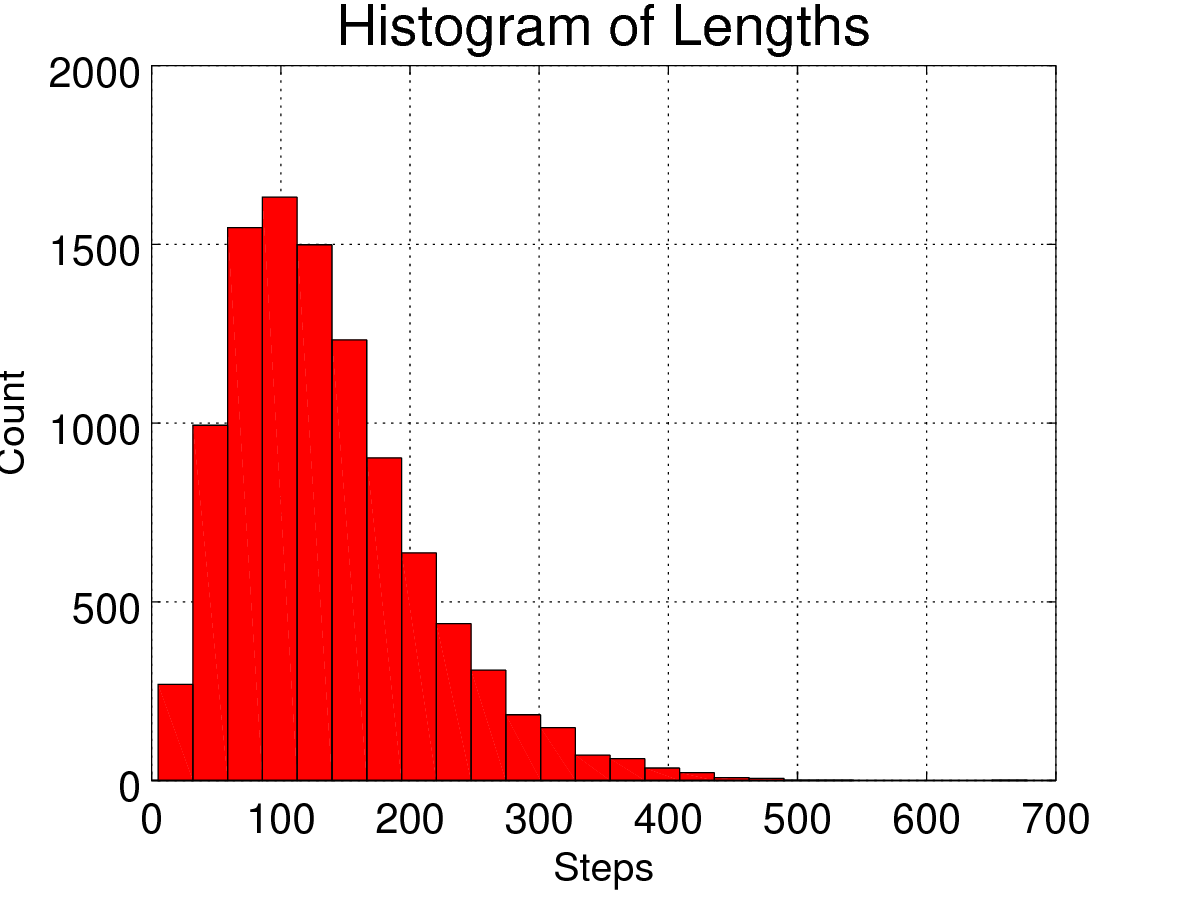
\includegraphics[width=0.95\textwidth]{figures/extraCredit/withHole_N10000.png}
    \caption{Histogram of the number of steps required for a Rook to move from $(1,1)$ to all other corners back to $(1,1)$ on a board with a hole in the middle. $N=10,000$ sample paths taken (graph for extra credit).}
    \label{fig:extra_withHole}
\end{figure}

\subsection{Rook Path with Hole}
Just like the case without the hole in the middle of the board, we ran six cases to find the probability of the rook being on any valid square on the board. These plots can be found in Figure \ref{plots:graphs_5c1}. In the final plot run using $n=10,000,000$ steps, it is clear that not all squares have the same probability. Near the corners there is a noticeable rise in probability, the sides containing twelve squares have a decrease in probability and the sides containing only four squares are even lower. So there are three cases each with a slightly different probability. A few sample probabilities from each of these regions can be found in Table \ref{tab:region_probs}. The matrix final matrix of values for the probability distribution is in Equation \ref{eq:matrix_2} (data for the $n=10,000,000$ plot in Figure \ref{plots:graphs_5c1}).

\begin{equation}
    \label{eq:matrix_2}
     \begin{bmatrix}
   0.022730  & 0.022703 &  0.022607 &  0.012926 &  0.012999 &  0.022763 &  0.022735 &  0.022720 \\
   0.022659  & 0.022715 &  0.022654 &  0.012910 &  0.012989 &  0.022754 &  0.022645 &  0.022608\\
   0.014653  & 0.014625 &  0.014604 &  0.000000 &  0.000000 &  0.014671 &  0.014594 &  0.014620\\
   0.014630  & 0.014543 &  0.014567 &  0.000000 &  0.000000 &  0.014642 &  0.014598 &  0.014574\\
   0.014665  & 0.014667 &  0.014625 &  0.000000 &  0.000000 &  0.014635 &  0.014551 &  0.014550\\
   0.014660  & 0.014675 &  0.014617 &  0.000000 &  0.000000 &  0.014652 &  0.014547 &  0.014571\\
   0.022724  & 0.022744 &  0.022731 &  0.013038 &  0.012993 &  0.022878 &  0.022619 &  0.022710\\
   0.022818  & 0.022783 &  0.022717 &  0.013085 &  0.013031 &  0.022791 &  0.022768 &  0.022713\\
    \end{bmatrix}
\end{equation}

\begin{figure}
    \centering
    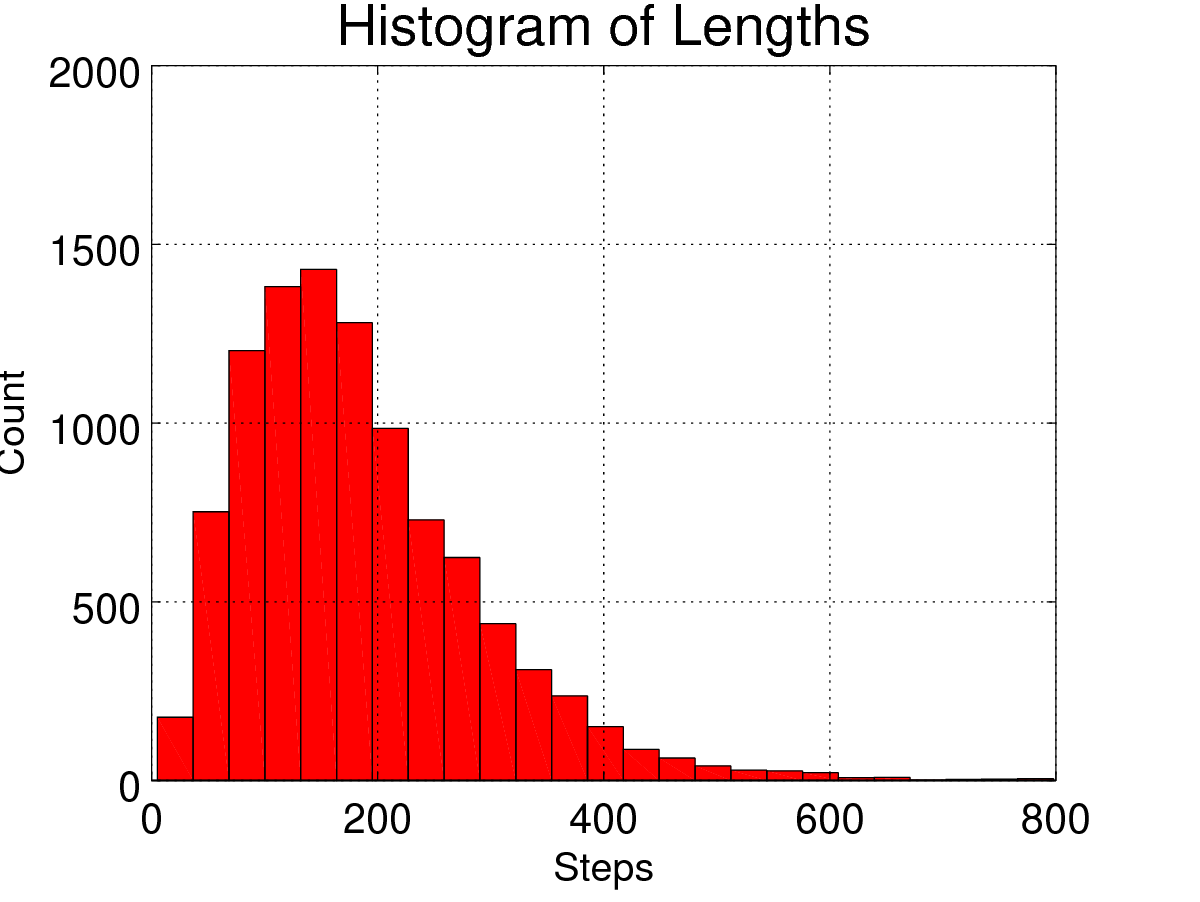
\includegraphics[width=0.95\textwidth]{figures/extraCredit/regular_N10000.png}
    \caption{Histogram of the number of steps required for a Rook to move from $(1,1)$ to all other corners back to $(1,1)$. $N=10,000$ sample paths taken (graph for extra credit).}
    \label{fig:extra_regular}
\end{figure}

\begin{table}[]
    \centering
    \begin{tabular}{|c|c|}
        \hline
        Type & Sample Probabilities \\
        \hline
        Red (four corners) & $0.022818$\\
        \hline
        Yellow (3X4 sides) & $0.014630$\\
        \hline
        Green (2X2 sides) & $0.012926$ \\
        \hline
    \end{tabular}
    \caption{The three categories of probabilities for the plots in Figure \ref{plots:graphs_5c1}.}
    \label{tab:region_probs}
\end{table}


\begin{table}[]
    \centering
    \begin{tabular}{|c|c|}
        \hline
        Type & Average number of Steps \\
        \hline
        Without hole & $186.1960$\\
        \hline
        With hole & $135.5228$\\
        \hline
    \end{tabular}
    \caption{Rook's average journey length from $(1,1)$ to all corners and then back to $(1,1)$.}
    \label{tab:avg_steps_journey2}
\end{table}

\begin{figure}
    \centering
    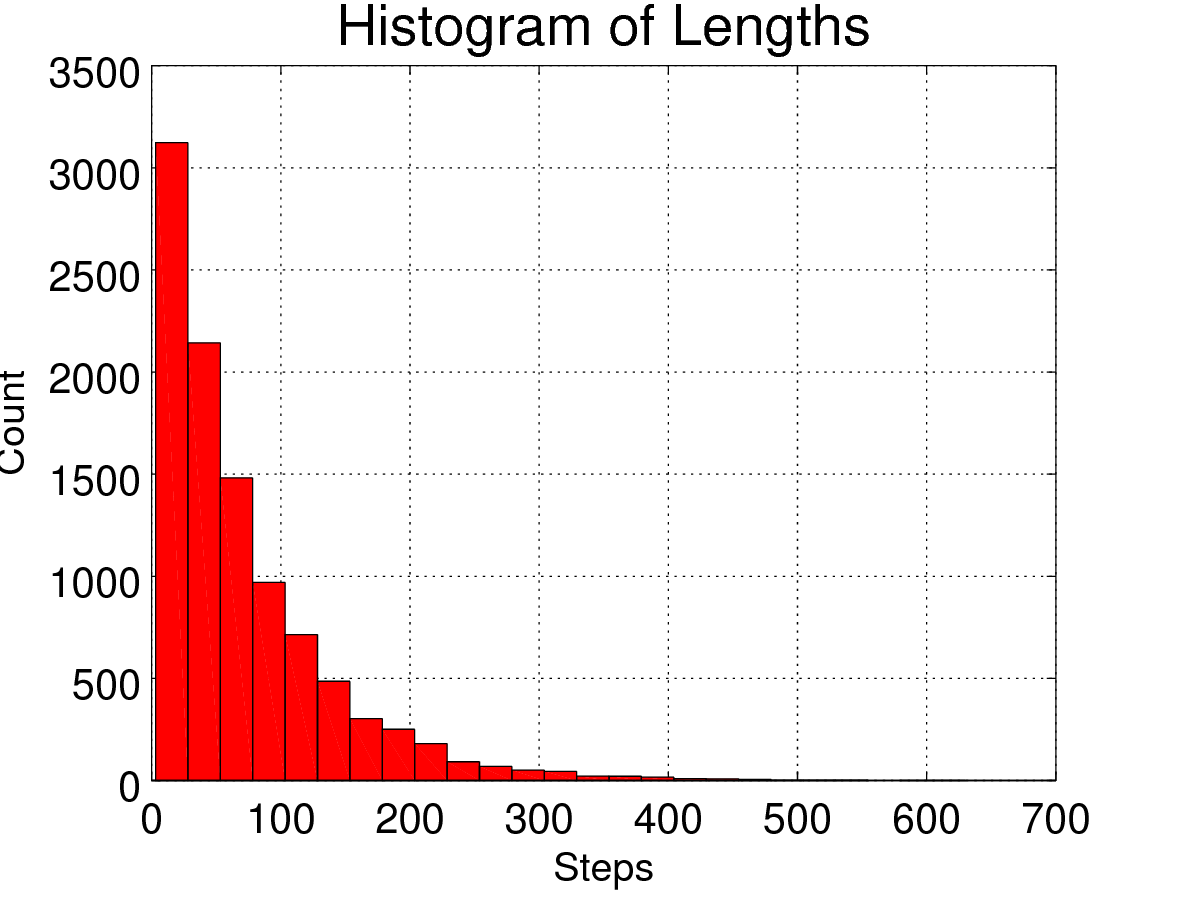
\includegraphics[width=0.95\textwidth]{figures/regular/figure_Rook_journey_N10000.png}
    \caption{Histogram of the number of steps required for a Rook to move from $(1,1)$ to $(8,8)$. $N=10,000$ sample paths taken (graph for 5b).}
    \label{plots:graphs_5b}
\end{figure}

\subsection{Rook Journey with Hole}
Again we preform $N=10,000$ samples paths to compute the average number of steps to perform the journey from $(1,1)$ to $(8,8)$, but this time with a hole in the middle of the board. The histogram of results can be found in Figure \ref{plots:graphs_5c2}. Here the distribution is skewed right. The average number of steps to perform this traversal is $54.3891$. The average number of steps to perform this journey is less than that for the case without the hole.

\begin{figure}
    \centering
    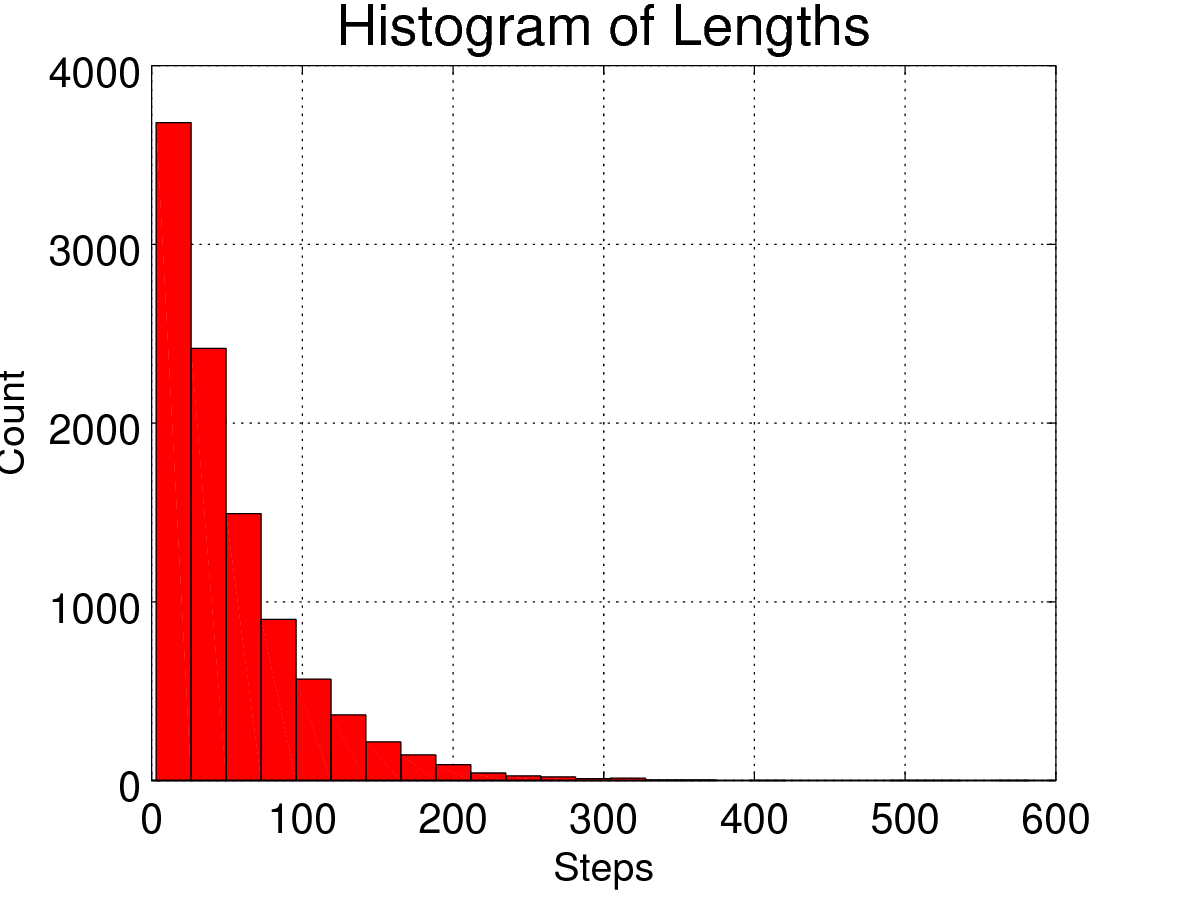
\includegraphics[width=0.95\textwidth]{figures/withHole/figure_Rook_journey_N10000.png}
    \caption{Histogram of the number of steps required for a Rook to move from $(1,1)$ to $(8,8)$ on a board with a hole in the middle. $N=10,000$ sample paths taken (graph for 5c).}
    \label{plots:graphs_5c2}
\end{figure}

\subsection{Rook Journey to all Corners (Extra Credit)}
We also computed average number of steps to touch all corners and come back to $(1,1)$. The noticeable difference in this case is that the distributions in Figures \ref{fig:extra_regular} and \ref{fig:extra_withHole} for the regular board and the board with the hole respectively, have been pushed a little to the right. These distributions are still skewed right, but not as much as the journey from $(1,1)$ to $(8,8)$. The average number of steps for the general case is $186.1960$ and when a hole is present the average is reduced to $135.5228$ steps. Adding in the hole makes the distribution of possible path lengths more peaked and than without the hole.


%Average steps from one corner to the opposite corner: $70.9033$ \par
%Average steps from one corner to the opposite corner with hole: $54.3891$ \par
%Average steps from one corner to all corners: $186.1960$ \par
%Average steps from one corner to all corners with hole: $135.5228$ \par


\section{Discussion}
The rook has equal probability of moving to any square on the board except when a hole is added into the mix. The result of adding the hole to a standard chessboard is that the rook has both fewer squares to move to and the corners have more options for movement than those on the sides. This can be seen in Figure \ref{plots:graphs_5c1} where the corners of the board are raised above the rest of the board. The reduction in squares and increase in the corner probabilities leads to the noticeable increase in speed for both of the journeys (see Tables \ref{tab:avg_steps} and \ref{tab:avg_steps_journey2}). An interesting observation is that if we divide the average step counts with the hole by the case without the hole we end up with two ratios that are very close to one another for the two journey types. The ratio for the corner to corner journey can be found in Equation \ref{eq:ratio_1} and the ratio for the corner to all corners journey can be found in Equation \ref{eq:ratio_2}.
\begin{equation}
    \label{eq:ratio_1}
    \frac{\text{with hole}}{\text{without hole}}=\frac{54.3891}{70.9033}\approx0.7671
\end{equation}
\begin{equation}
    \label{eq:ratio_2}
    \frac{\text{with hole}}{\text{without hole}}=\frac{135.5228}{186.1960}\approx0.7279
\end{equation}
This might just be a coincidence, but it could be that the two journeys are effected by the addition of the hole in the same way. \par
Looking at the histograms for both of the journeys made without a hole (Figures \ref{plots:graphs_5b} and \ref{fig:extra_regular}) it is clear that forcing the rook to journey to all corners and then back to the starting corner does shift the distribution to right. The Journey across the board is attracted to smaller step counts while the journey to all corners is centered around $125$. \par

The data we collected could be well compared to what we would have otherwise thought would happen because there are only so many locations you can come from to reach a single point on a chessboard with the constraints we have placed by using a Rook. Only being able to move vertically or horizontally creates a limit of positions to move from to get to one spot. At most, with the full board there are equally as many points to come from as there are from position to position. This will give us an even distribution on an open board of about 1/14th of a chance to land on any position from any of the positions along the paths allowable. Coincidentally, if we are looking at the board with the hole, there are a varying amount of positions from several positions to the location we try to get to. If we wanted to know the percent distribution before running the code, we could have added up the amount of how many paths could lead to each of the positions on the new board with a hole and that would have given us our distribution.



\section{Conclusions}
The rook can move to any position on a standard chessboard with equal probability which in turn means it has equal probability of existing on any given square. At each square on the chessboard the rook can move to exactly $14$ positions, leading to an equal probability for each square. When traveling across the board from one corner to the opposite corner the rook takes on average $71$ steps (rounding to nearest whole number). When a hole is added to the board the average number of steps decreases because there are fewer places the rook can move to and the probability for the corners increases relative to the sides. The hole we added to the board was from C4-F4 and C5-F5; this reduced the number of steps to $54$. These same two cases can be run using a modified journey in which the rook moves to all corners and then back to its starting corner. Again, we find an overall reduction in the average step counts from $186$ steps to $136$ steps. Adding in the hole changed the dynamics of the board from an equal probability distribution to the distribution found in Figure \ref{plots:graphs_5c1}. \par
In the future it might be interesting to see how increasing the size of the board might effect the average number of steps it takes to perform a traversal from one corner to another corner. Comparing the average steps for say 8X8, 16X16, 32X32 and so on might produce some interesting scaling factors that we could use to predict the average number of steps for larger boards. Other areas of interest include adding different size holes to the board, biasing the movement of the rook, and performing more journeys such as touching every point down the diagonal paths of the board.

\section{Extra Credit}
Talked about in section 3.6.

\newpage
\section{Attachments}

\begin{figure}[!h]
    \centering
   \begin{minipage}{0.50\textwidth}
     \centering
     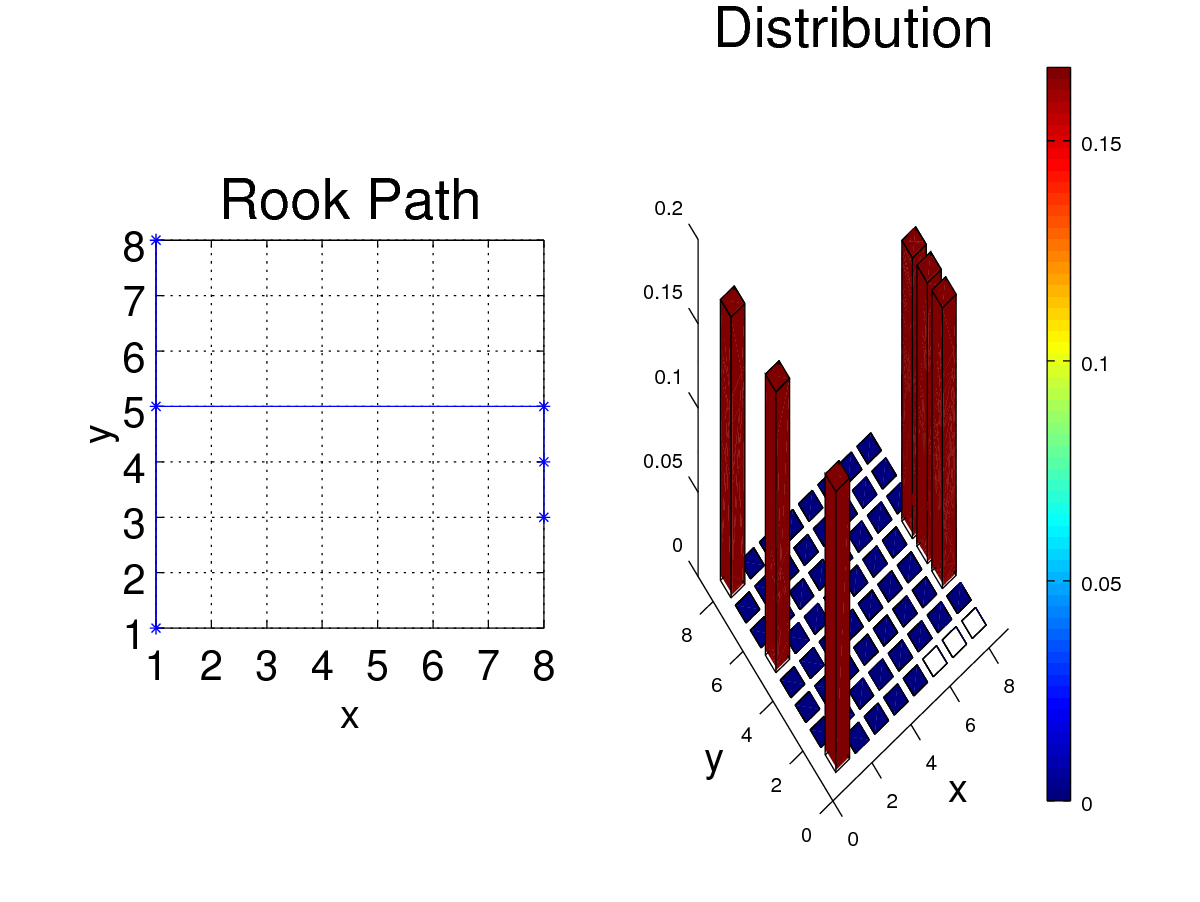
\includegraphics[width=1.0\linewidth]{figures/regular/figure_Rook_path_n5_x1_y1.png}
     \captionsetup{labelformat=empty}
     \caption*{$n=5$}
   \end{minipage}\hfil
   \begin{minipage}{0.50\textwidth}
     \centering
     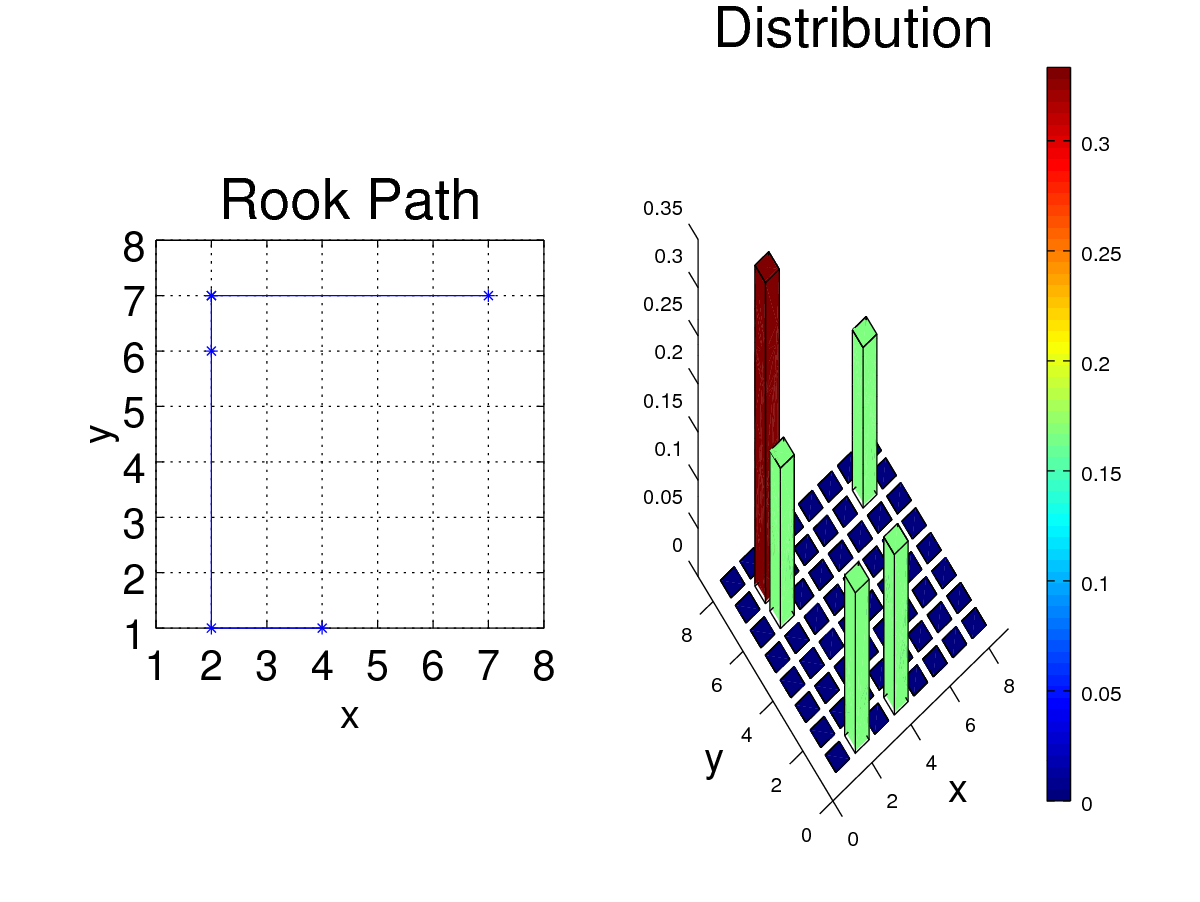
\includegraphics[width=1.0\linewidth]{figures/regular/figure_Rook_path_n5_x4_y1.png}
     \captionsetup*{labelformat=empty}
     \caption{$n=5$}
   \end{minipage}\hfil
   \begin{minipage}{0.50\textwidth}
     \centering
     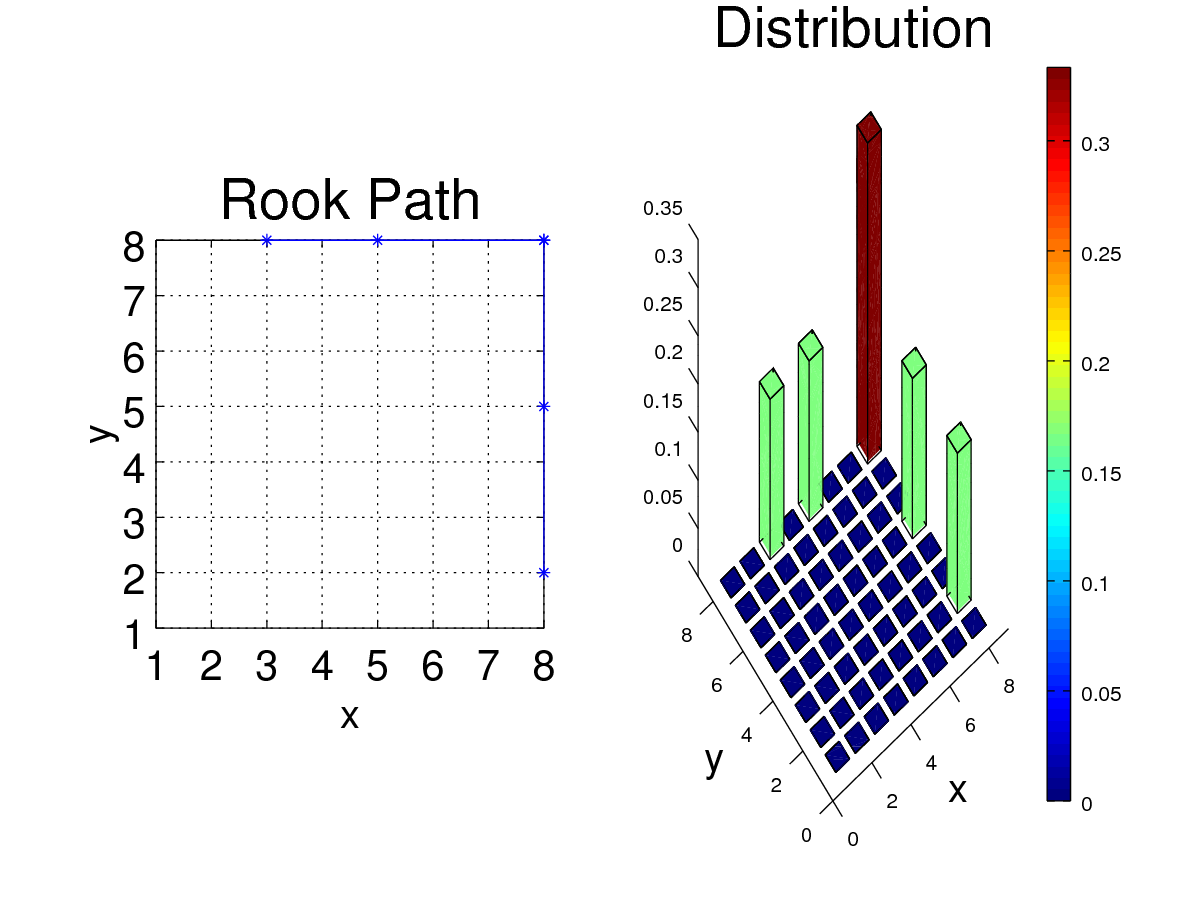
\includegraphics[width=1.0\linewidth]{figures/regular/figure_Rook_path_n5_x8_y8.png}
     \captionsetup{labelformat=empty}
     \caption*{$n=5$}
    \end{minipage}\hfil
    \begin{minipage}{0.50\textwidth}
     \centering
     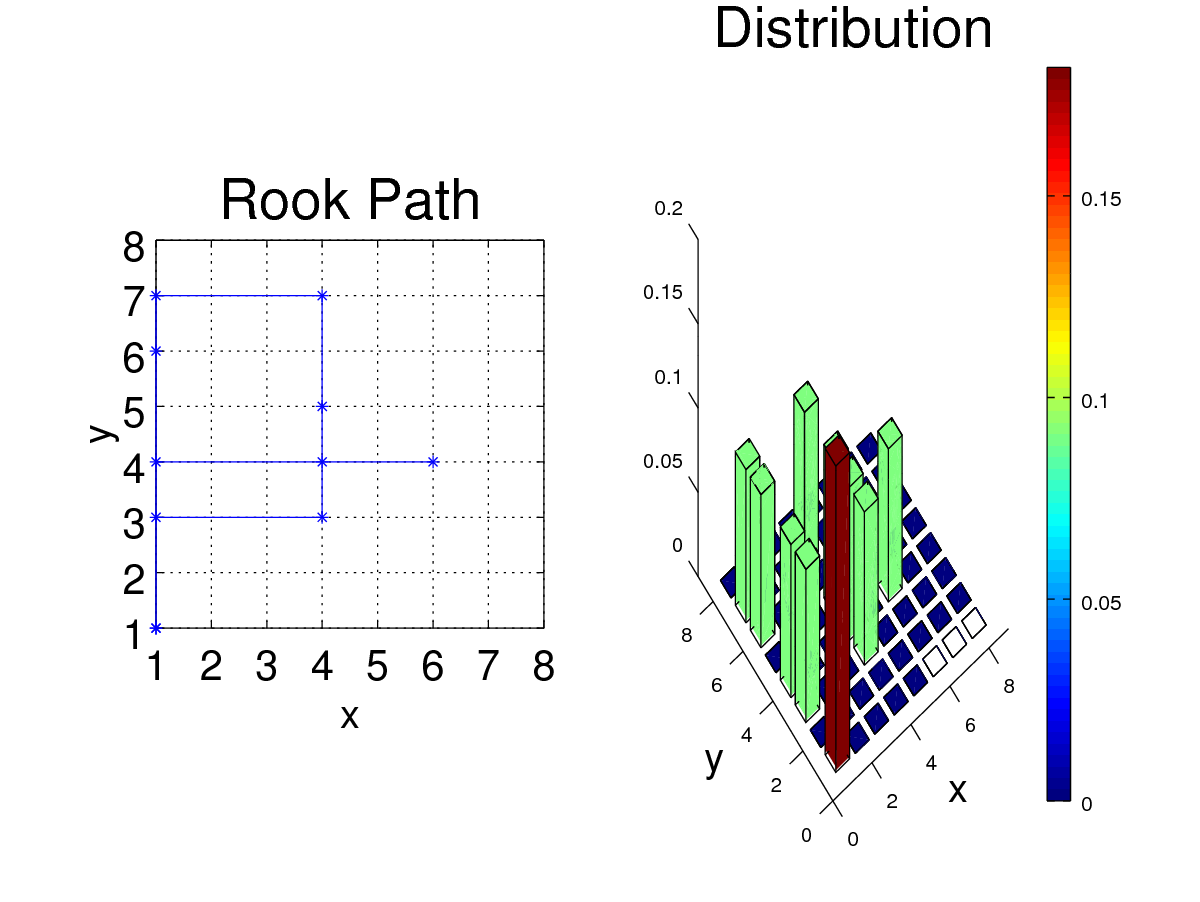
\includegraphics[width=1.0\linewidth]{figures/regular/figure_Rook_path_n10_x1_y1.png}
     \captionsetup{labelformat=empty}
     \caption*{$n=10$}
   \end{minipage}\hfil
   \begin{minipage}{0.50\textwidth}
     \centering
     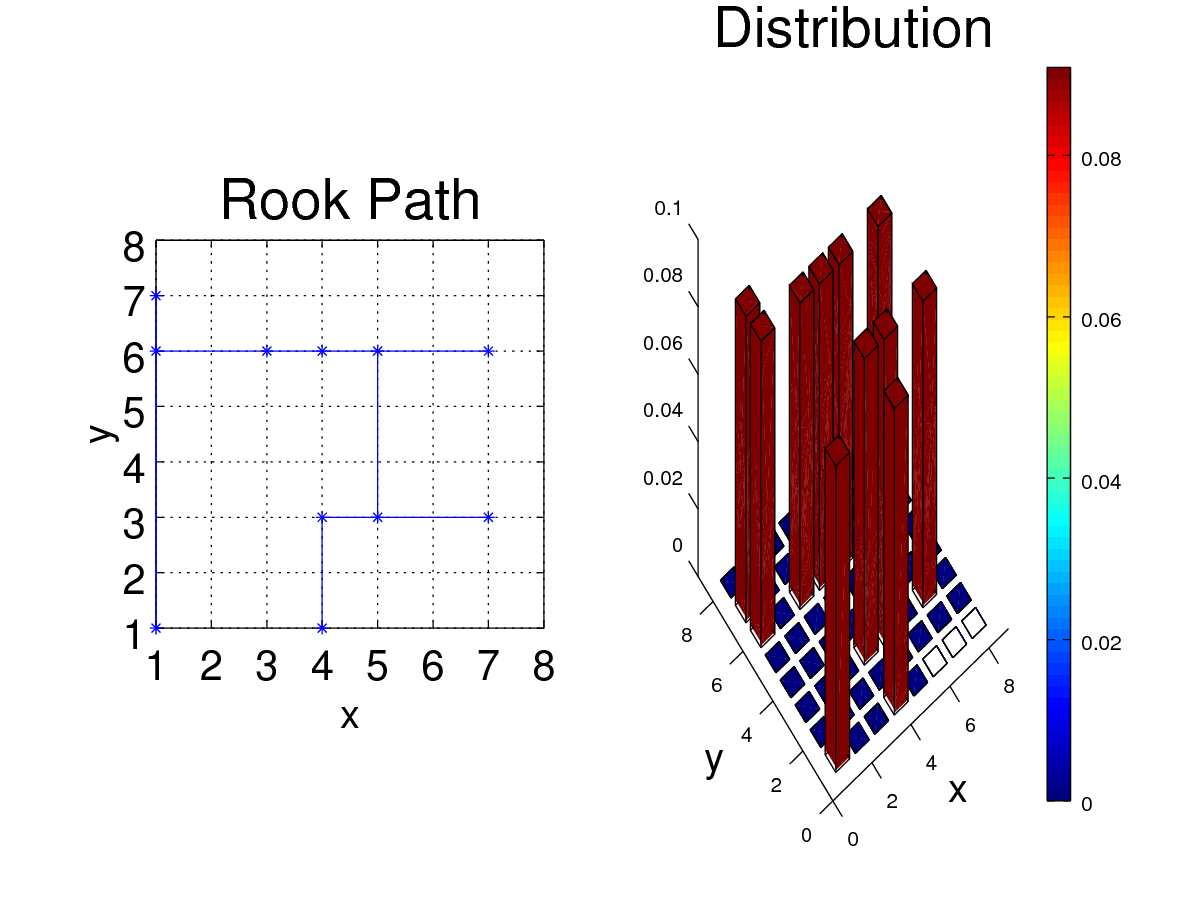
\includegraphics[width=1.0\linewidth]{figures/regular/figure_Rook_path_n10_x4_y1.png}
     \captionsetup*{labelformat=empty}
     \caption{$n=10$}
   \end{minipage}\hfil
   \begin{minipage}{0.50\textwidth}
     \centering
     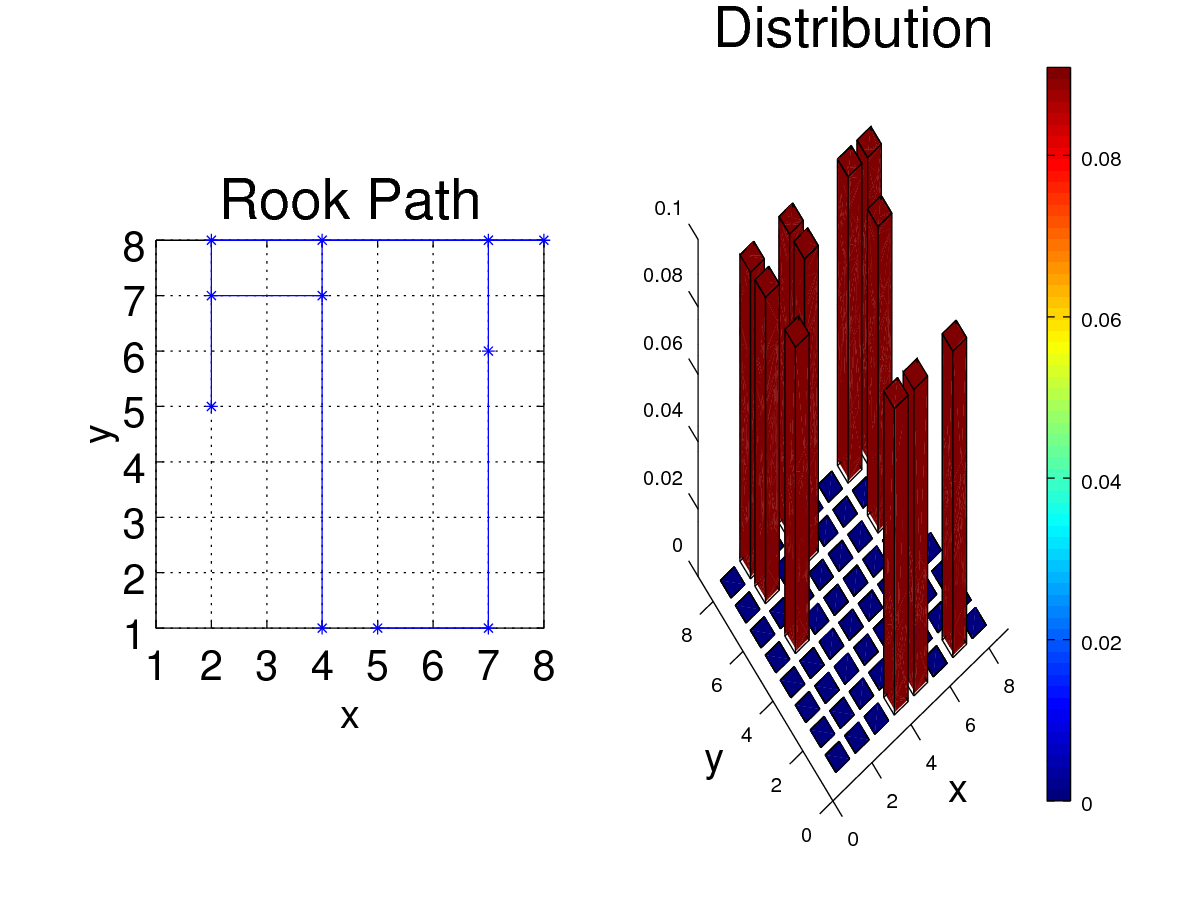
\includegraphics[width=1.0\linewidth]{figures/regular/figure_Rook_path_n10_x8_y8.png}
     \captionsetup{labelformat=empty}
     \caption*{$n=10$}
    \end{minipage}\hfil
    %\captionsetup{labelformat=empty}
    \caption{A few example paths without a hole in the board.}
    \label{plots:graphs_paths_regular}
\end{figure}

\begin{figure}[!h]
    \centering
   \begin{minipage}{0.50\textwidth}
     \centering
     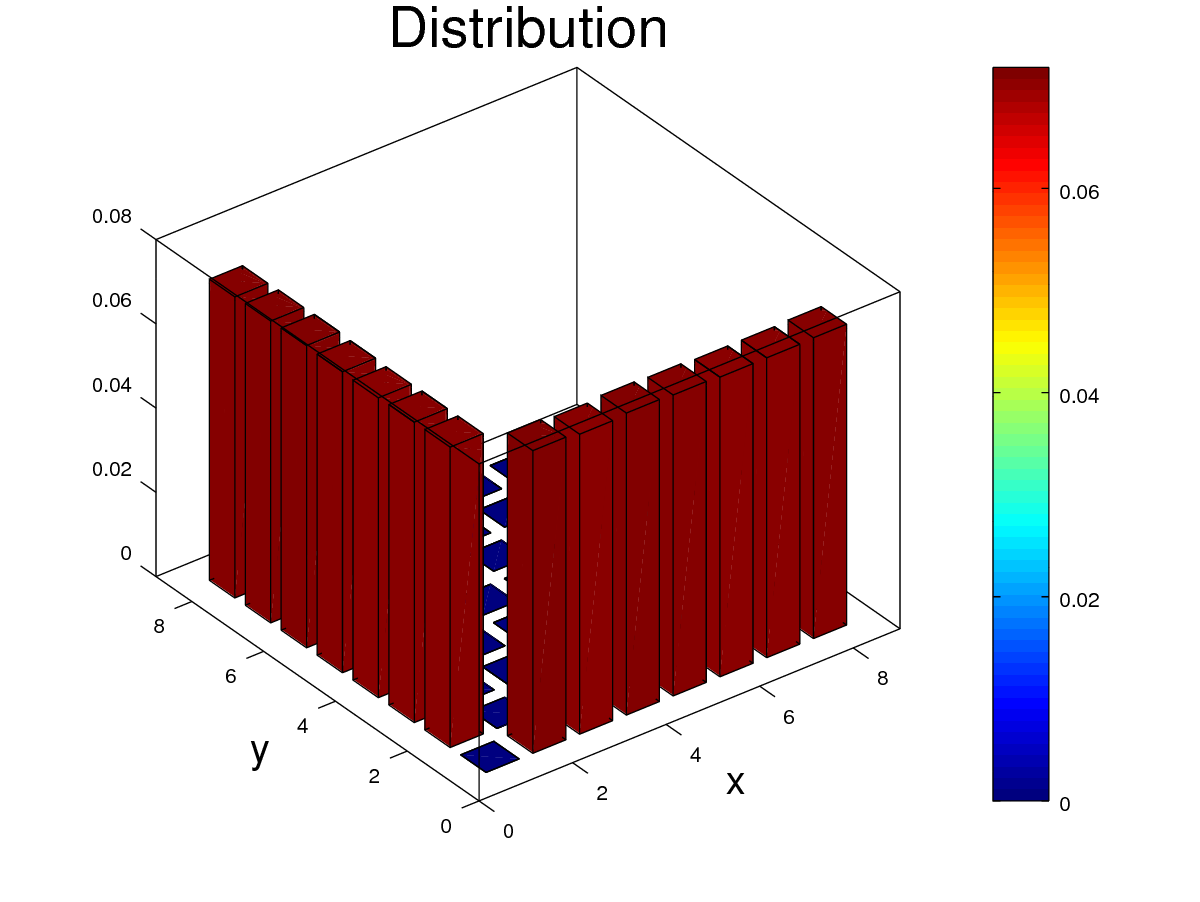
\includegraphics[width=1.0\linewidth]{figures/regular/figure_Rook_moveFixedOrigin_N1000000_x1_y1.png}
     \captionsetup{labelformat=empty}
     \caption*{$n=1,000,000$}
   \end{minipage}\hfil
   \begin{minipage}{0.50\textwidth}
     \centering
     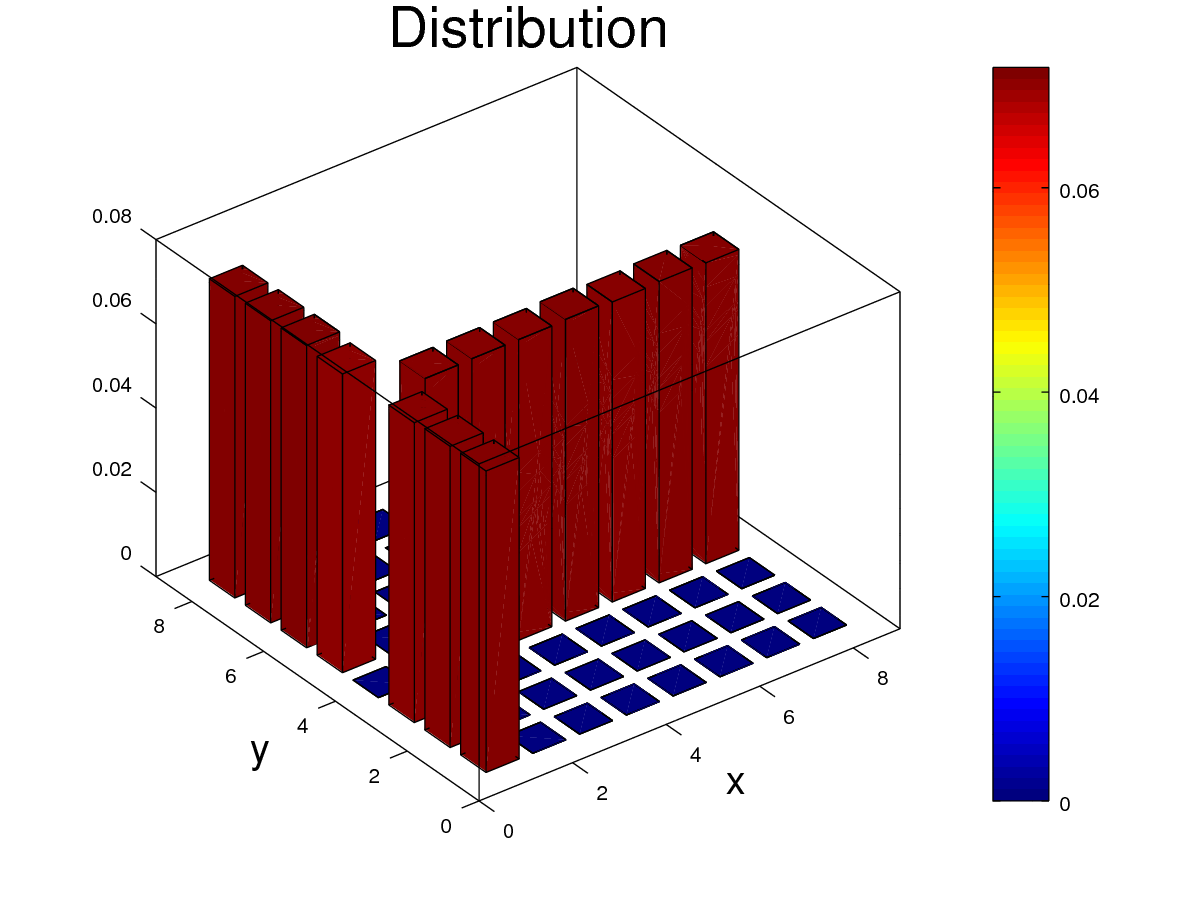
\includegraphics[width=1.0\linewidth]{figures/regular/figure_Rook_moveFixedOrigin_N1000000_x1_y4.png}
     \captionsetup*{labelformat=empty}
     \caption{$n=1,000,000$}
   \end{minipage}\hfil
   \begin{minipage}{0.50\textwidth}
     \centering
     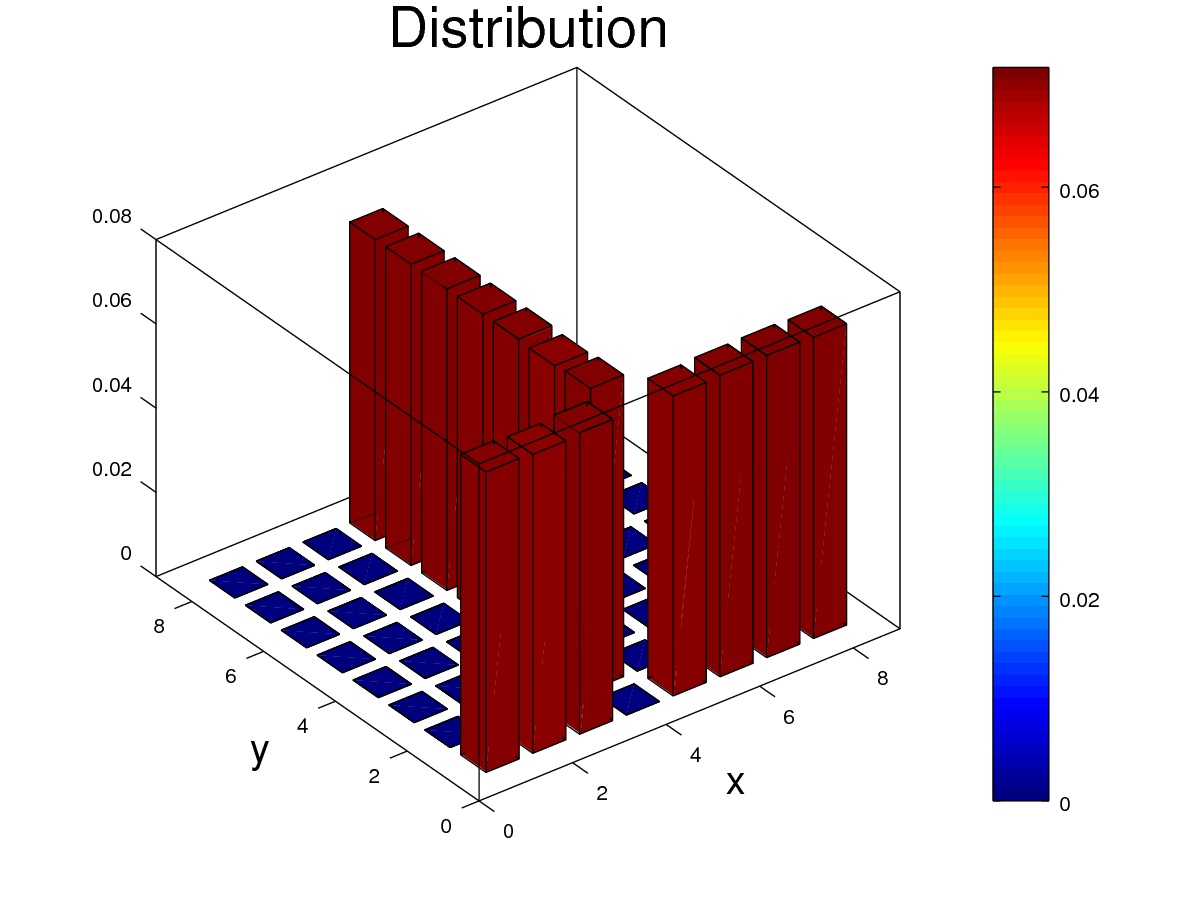
\includegraphics[width=1.0\linewidth]{figures/regular/figure_Rook_moveFixedOrigin_N1000000_x4_y1.png}
     \captionsetup{labelformat=empty}
     \caption*{$n=1,000,000$}
    \end{minipage}\hfil
    \begin{minipage}{0.50\textwidth}
     \centering
     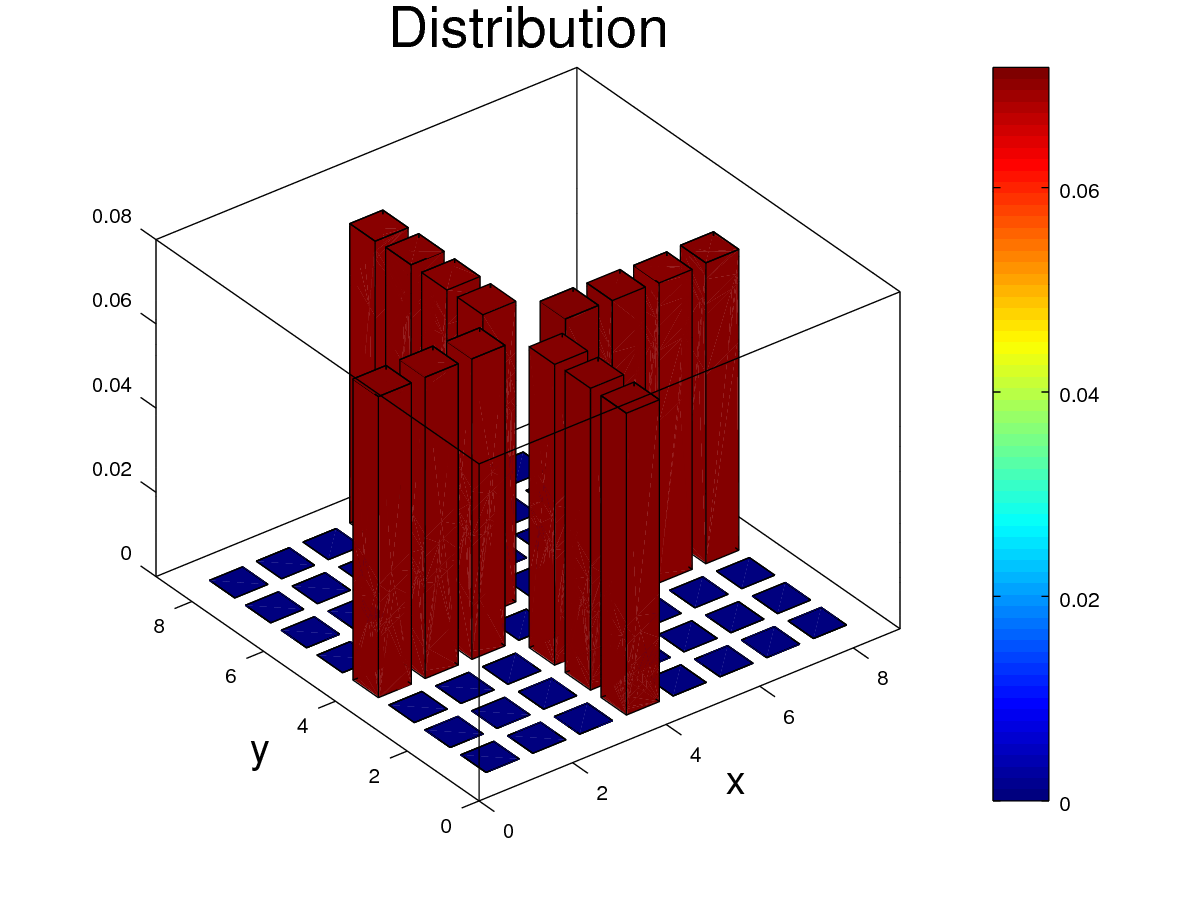
\includegraphics[width=1.0\linewidth]{figures/regular/figure_Rook_moveFixedOrigin_N1000000_x4_y4.png}
     \captionsetup{labelformat=empty}
     \caption*{$n=1,000,000$}
   \end{minipage}\hfill
   \begin{minipage}{0.50\textwidth}
     \centering
     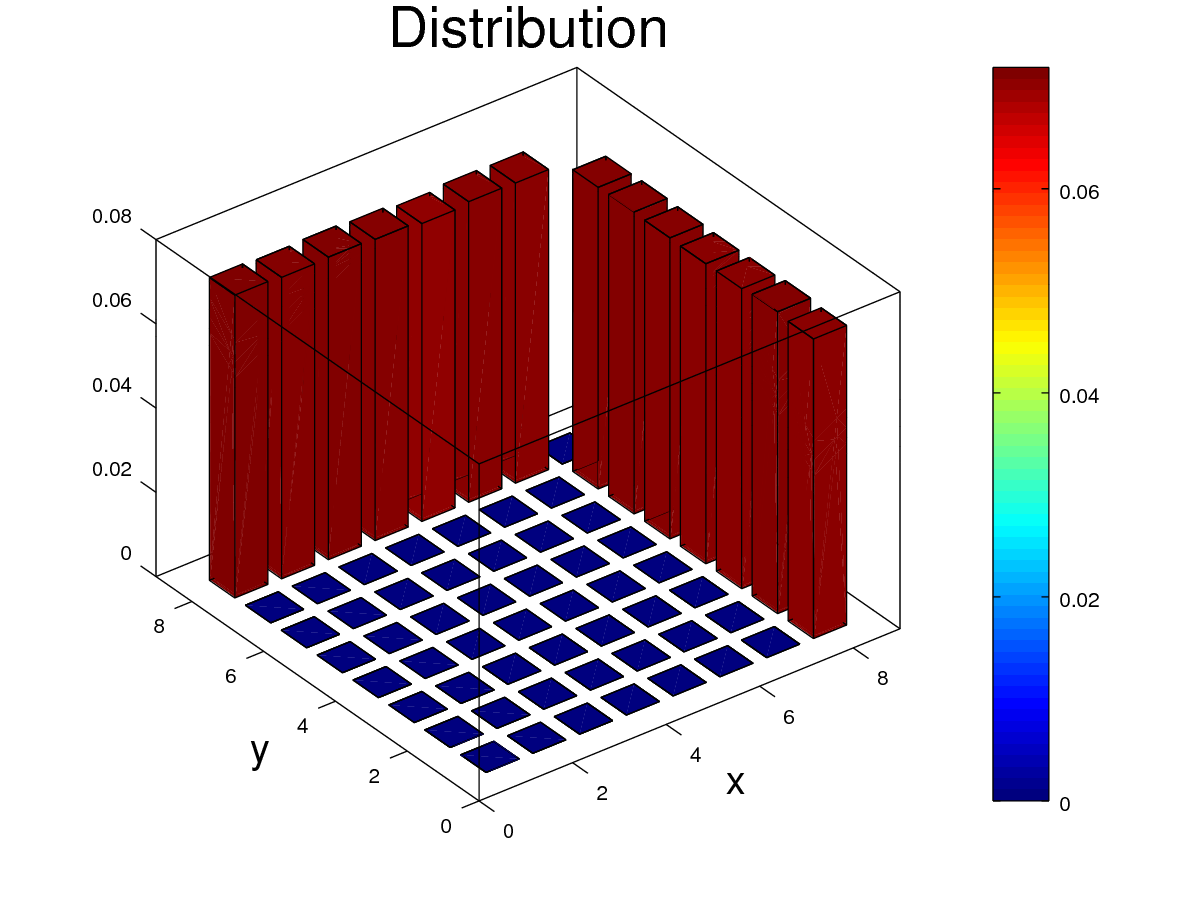
\includegraphics[width=1.0\linewidth]{figures/regular/figure_Rook_moveFixedOrigin_N1000000_x8_y8.png}
     \captionsetup{labelformat=empty}
     \caption*{$n=1,000,000$}
   \end{minipage}\hfil
    %\captionsetup{labelformat=empty}
    \caption{Test for the movement of the Rook without a hole in the board.}
    \label{plots:graphs_testing_regular}
\end{figure}

\begin{figure}[!h]
    \centering
   \begin{minipage}{0.50\textwidth}
     \centering
     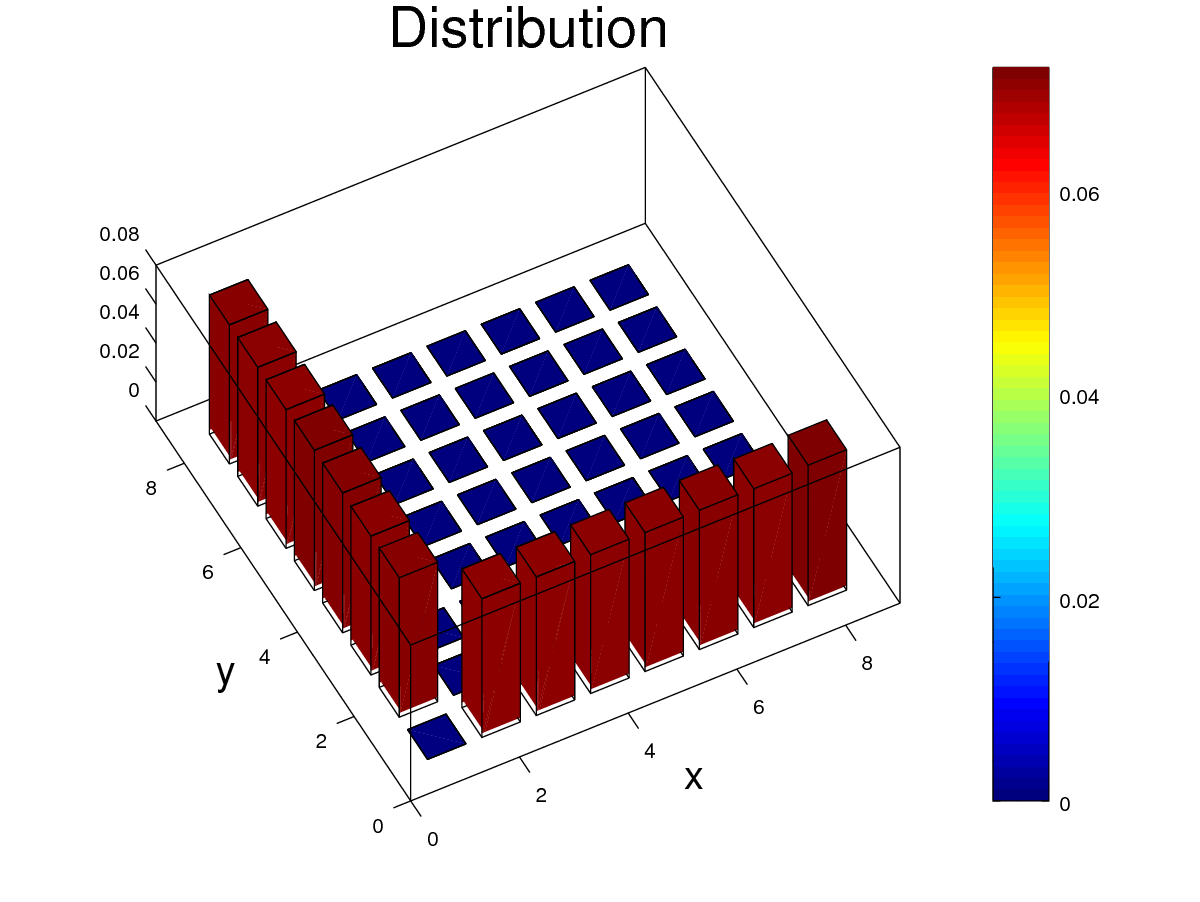
\includegraphics[width=1.0\linewidth]{figures/withHole/figure_Rook_moveFixedOrigin_N1000000_x1_y1.png}
     \captionsetup{labelformat=empty}
     \caption*{$n=1,000,000$}
   \end{minipage}\hfil
   \begin{minipage}{0.50\textwidth}
     \centering
     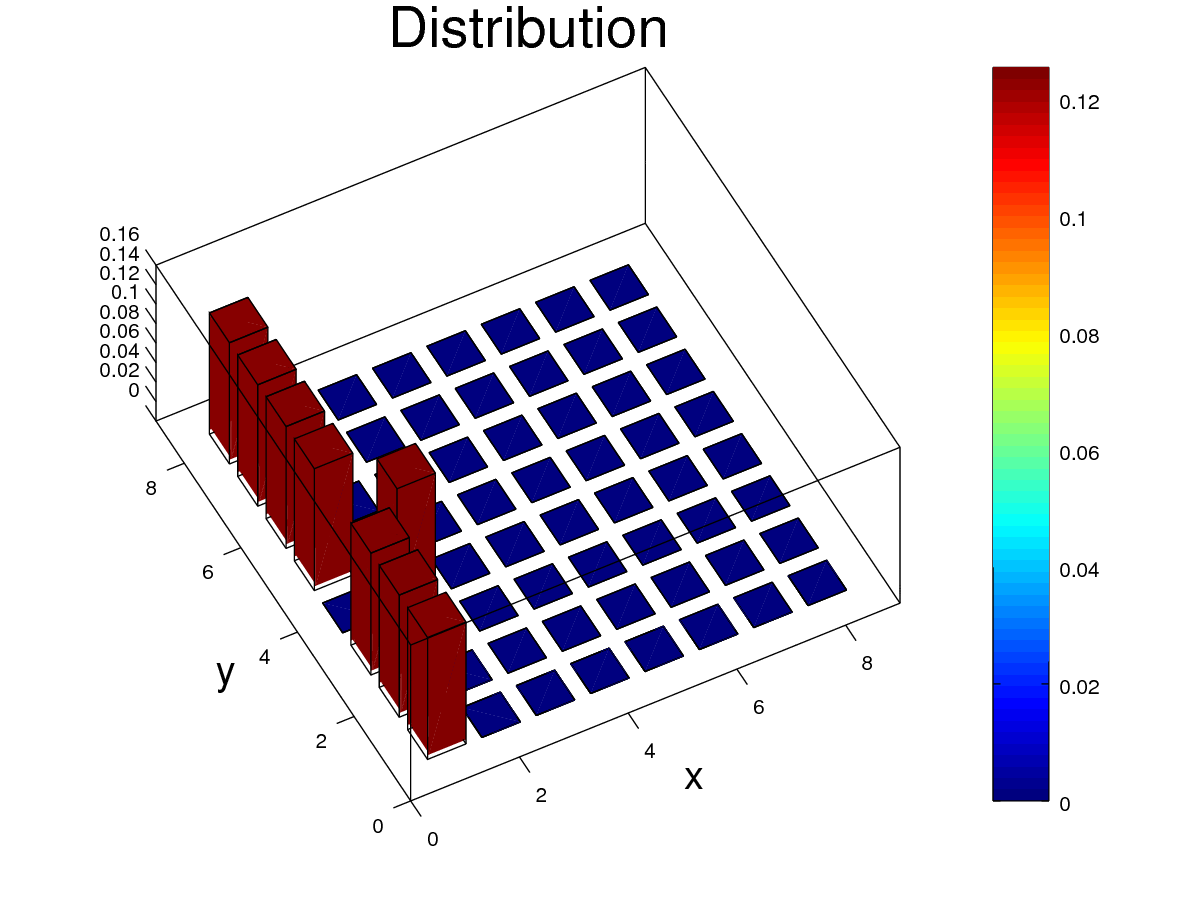
\includegraphics[width=1.0\linewidth]{figures/withHole/figure_Rook_moveFixedOrigin_N1000000_x1_y4.png}
     \captionsetup{labelformat=empty}
     \caption*{$n=1,000,000$}
   \end{minipage}\hfil
   \begin{minipage}{0.50\textwidth}
     \centering
     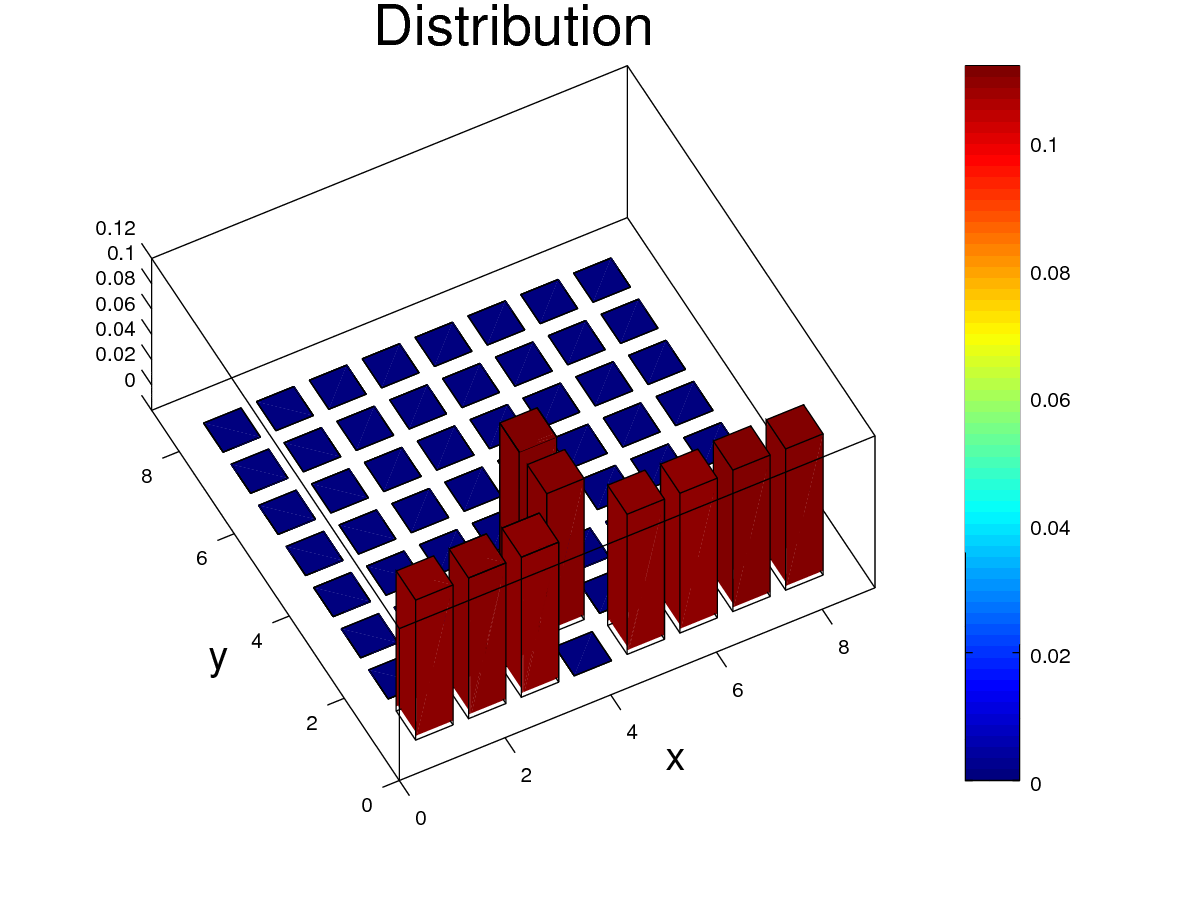
\includegraphics[width=1.0\linewidth]{figures/withHole/figure_Rook_moveFixedOrigin_N1000000_x4_y1.png}
     \captionsetup{labelformat=empty}
     \caption*{$n=1,000,000$}
    \end{minipage}\hfil
   \begin{minipage}{0.50\textwidth}
     \centering
     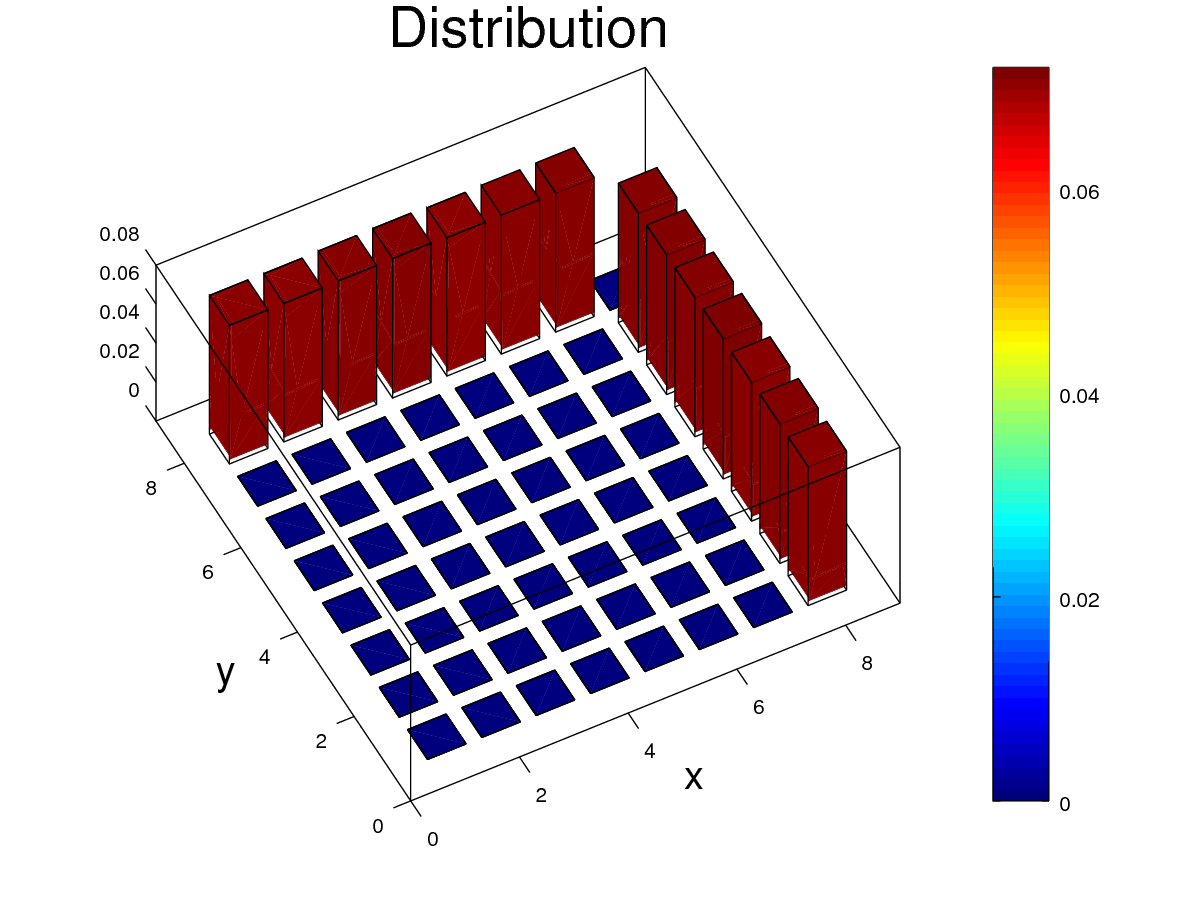
\includegraphics[width=1.0\linewidth]{figures/withHole/figure_Rook_moveFixedOrigin_N1000000_x8_y8.png}
     \captionsetup{labelformat=empty}
     \caption*{$n=1,000,000$}
   \end{minipage}\hfil
    %\captionsetup{labelformat=empty}
    \caption{Test for the movement of the rook with a hole.}
    \label{plots:graphs_testing_withHole}
\end{figure}

\begin{figure}[!h]
    \centering
   \begin{minipage}{0.50\textwidth}
     \centering
     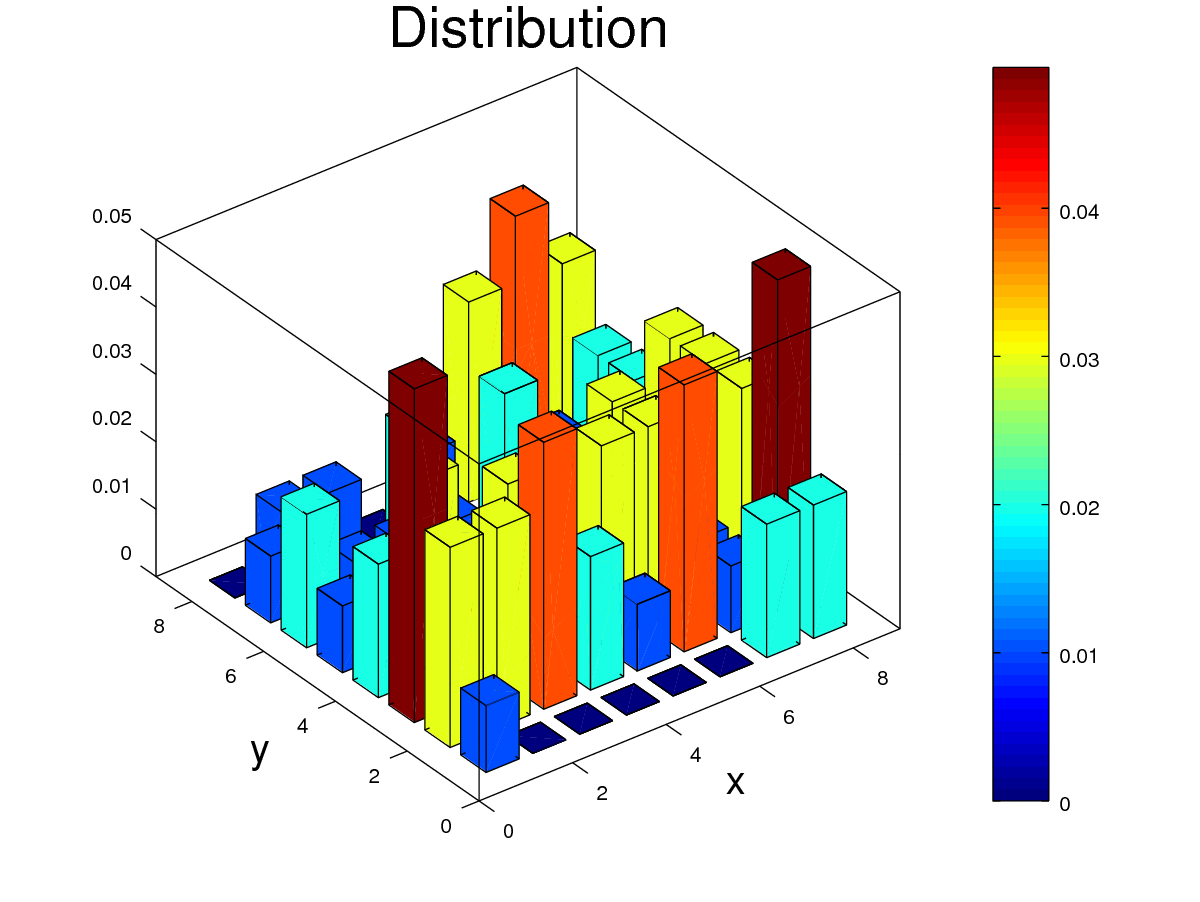
\includegraphics[width=1.0\linewidth]{figures/regular/figure_Rook_path_n100.png}
     \captionsetup{labelformat=empty}
     \caption*{$n=100$}
   \end{minipage}\hfil
   \begin{minipage}{0.50\textwidth}
     \centering
     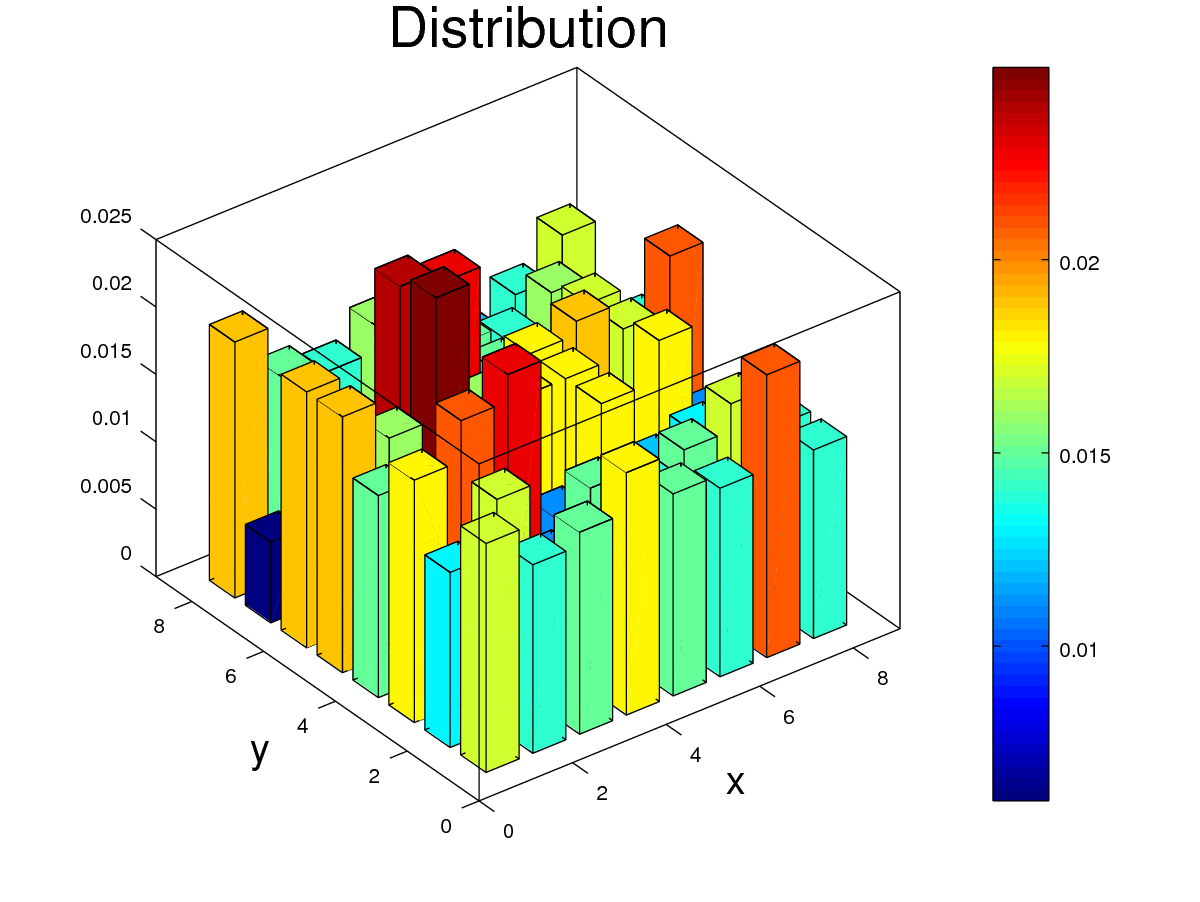
\includegraphics[width=1.0\linewidth]{figures/regular/figure_Rook_path_n1000.png}
     \captionsetup*{labelformat=empty}
     \caption{$n=1,000$}
   \end{minipage}\hfil
   \begin{minipage}{0.50\textwidth}
     \centering
     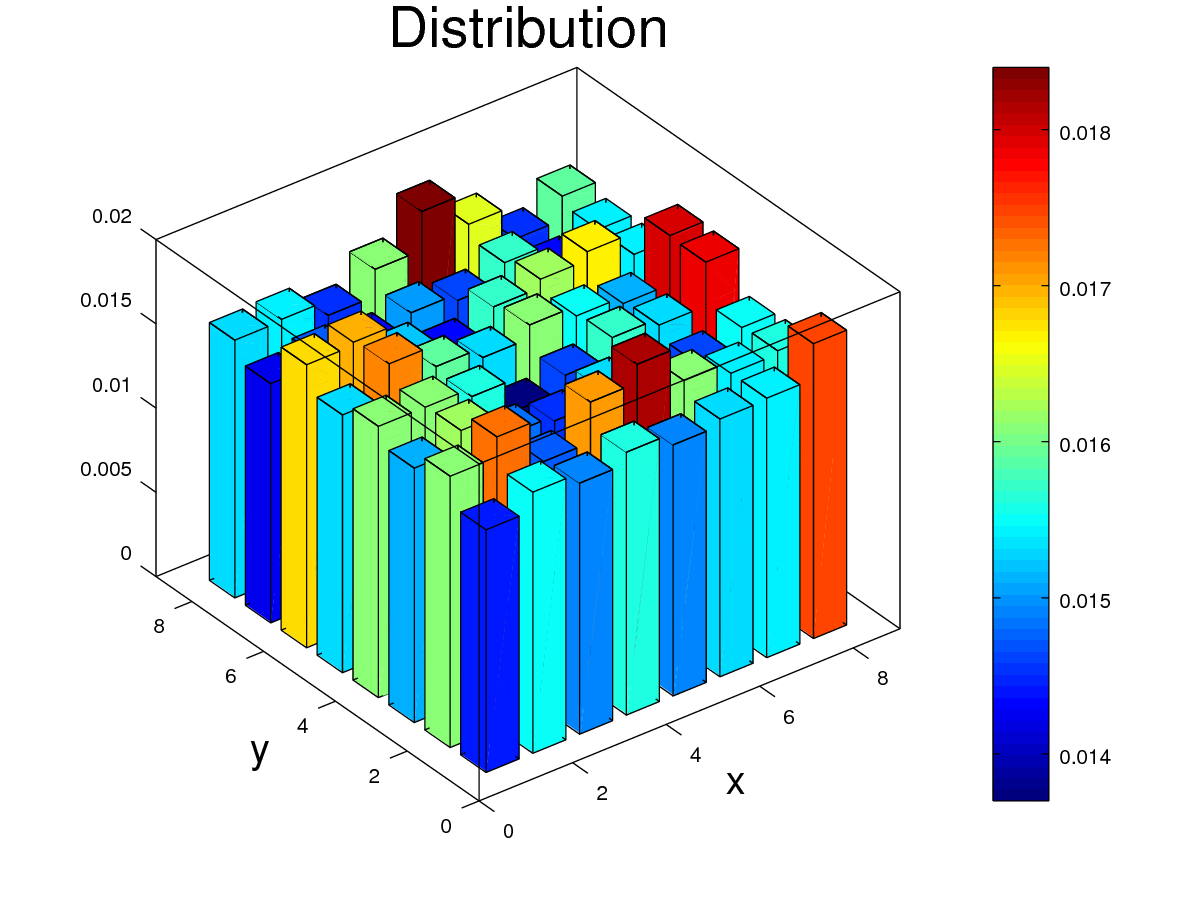
\includegraphics[width=1.0\linewidth]{figures/regular/figure_Rook_path_n10000.png}
     \captionsetup{labelformat=empty}
     \caption*{$n=10,000$}
    \end{minipage}\hfil
    \begin{minipage}{0.50\textwidth}
     \centering
     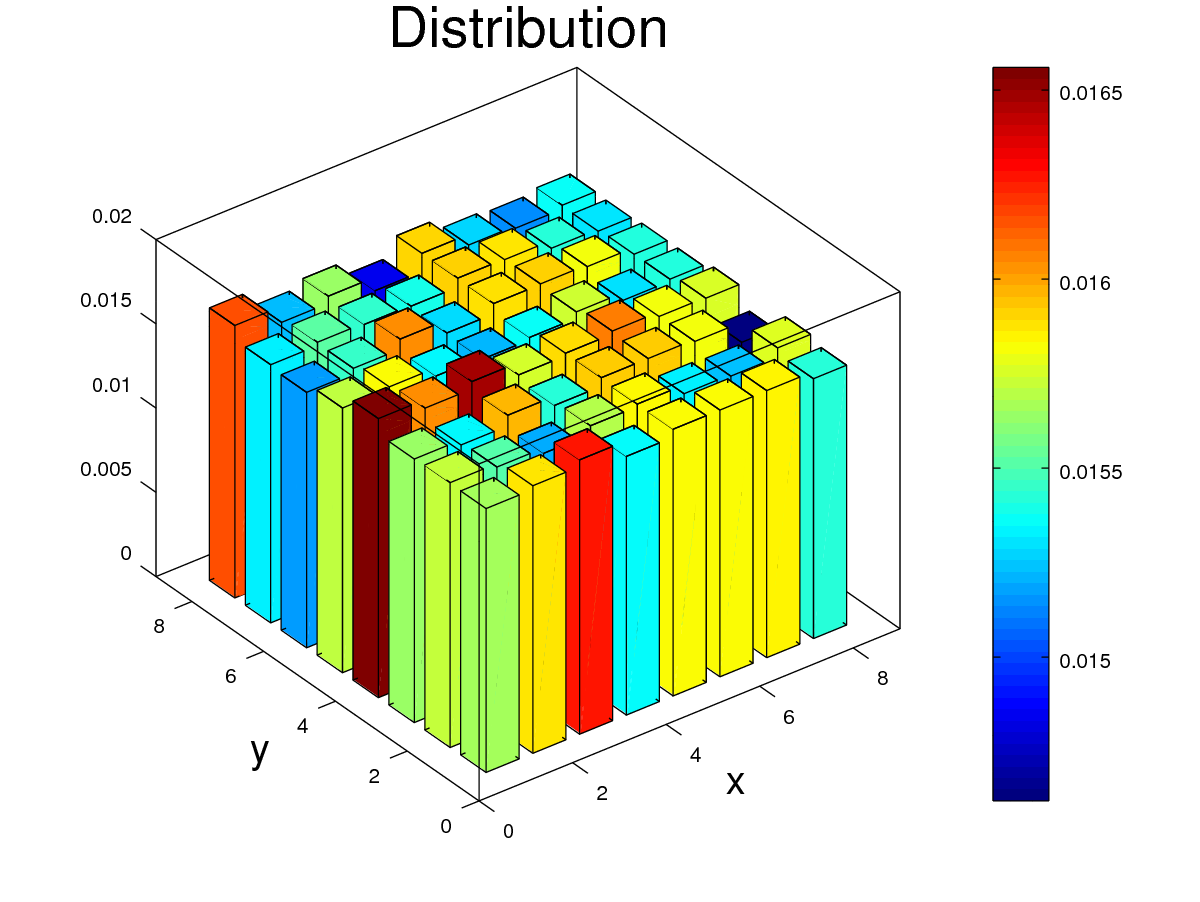
\includegraphics[width=1.0\linewidth]{figures/regular/figure_Rook_path_n100000.png}
     \captionsetup{labelformat=empty}
     \caption*{$n=100,000$}
   \end{minipage}\hfill
   \begin{minipage}{0.50\textwidth}
     \centering
     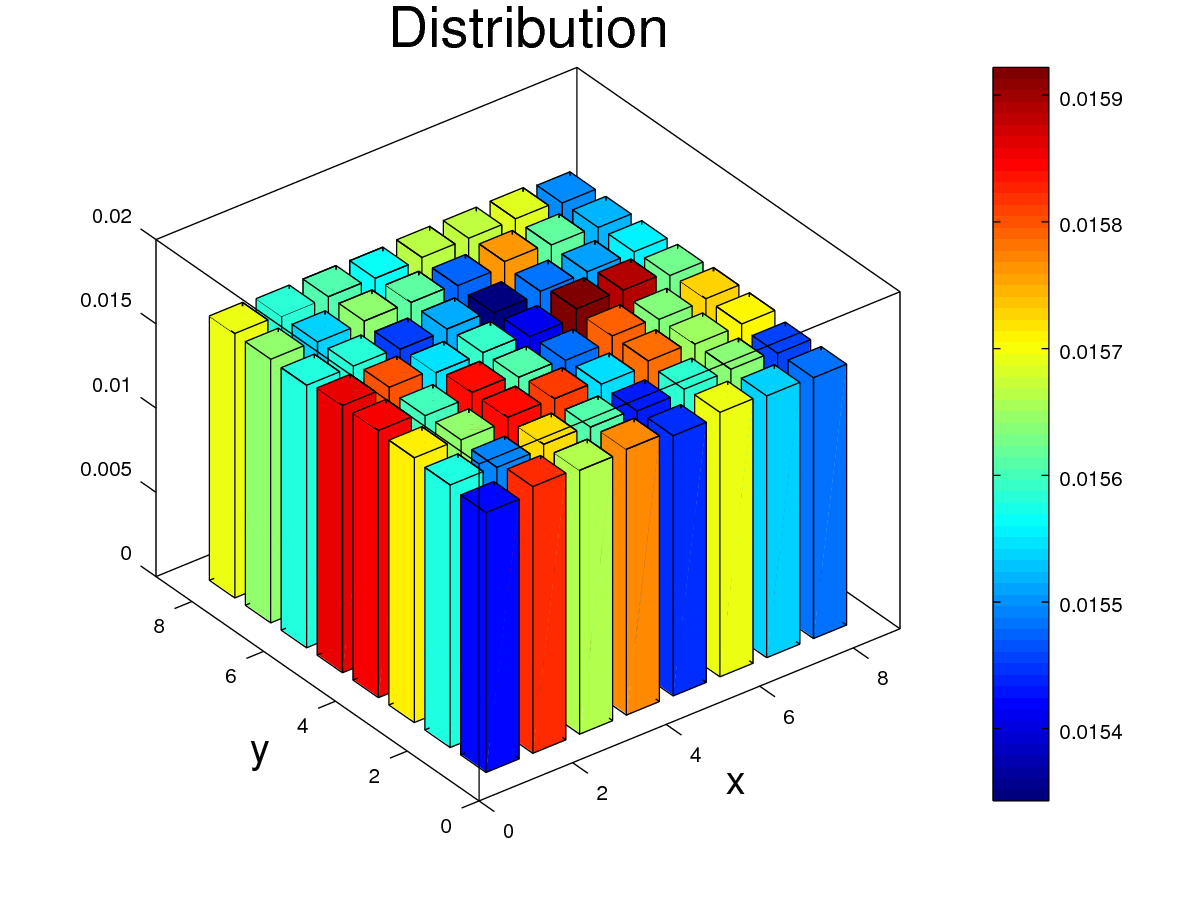
\includegraphics[width=1.0\linewidth]{figures/regular/figure_Rook_path_n1000000.png}
     \captionsetup{labelformat=empty}
     \caption*{$n=1,000,000$}
   \end{minipage}\hfil
   \begin{minipage}{0.50\textwidth}
     \centering
     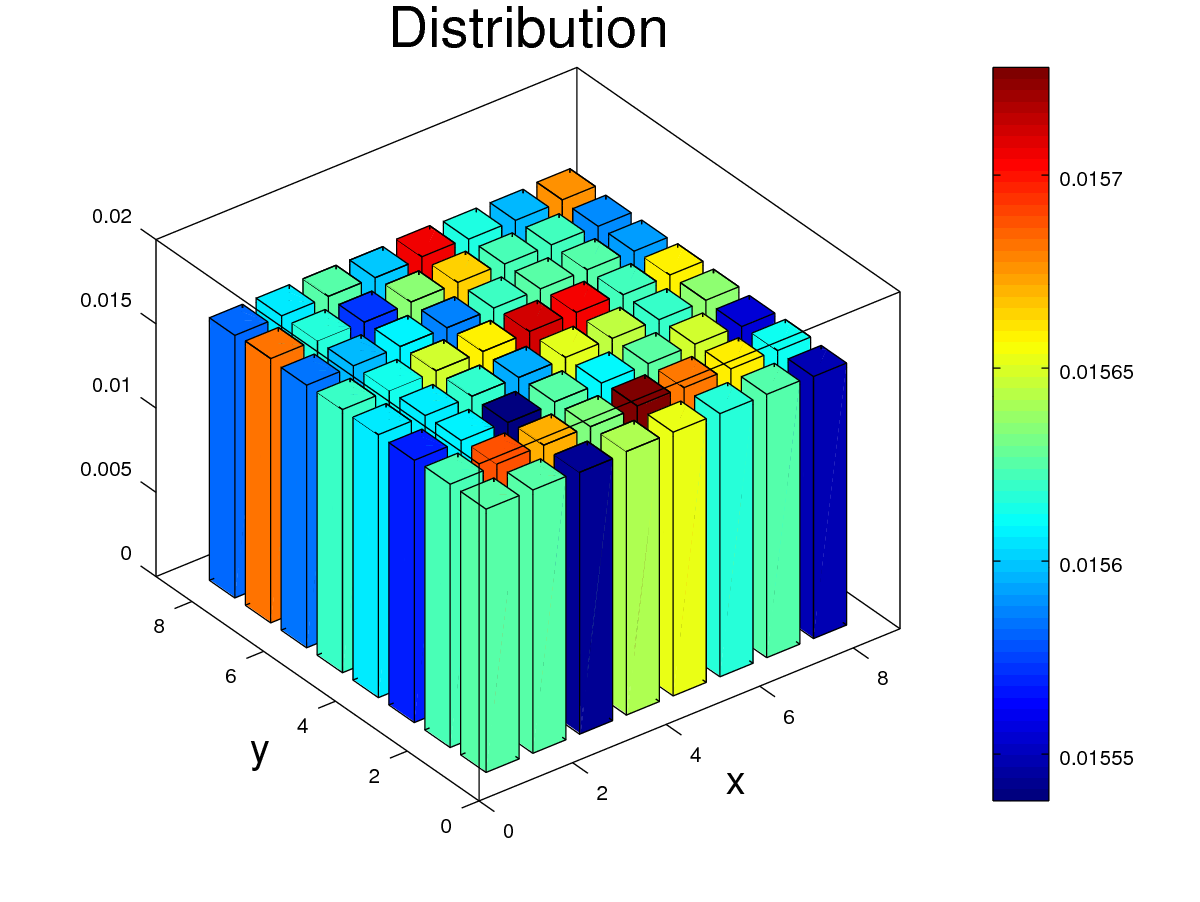
\includegraphics[width=1.0\linewidth]{figures/regular/figure_Rook_path_n10000000.png}
     \captionsetup{labelformat=empty}
     \caption*{$n=10,000,000$}
    \end{minipage}\hfil
    %\captionsetup{labelformat=empty}
    \caption{Graphs of the probability distribution of the Rook; each square on the board is represented by a column (graphs for 5a).}
    \label{plots:graphs_5a}
\end{figure}


\begin{figure}[!h]
    \centering
   \begin{minipage}{0.50\textwidth}
     \centering
     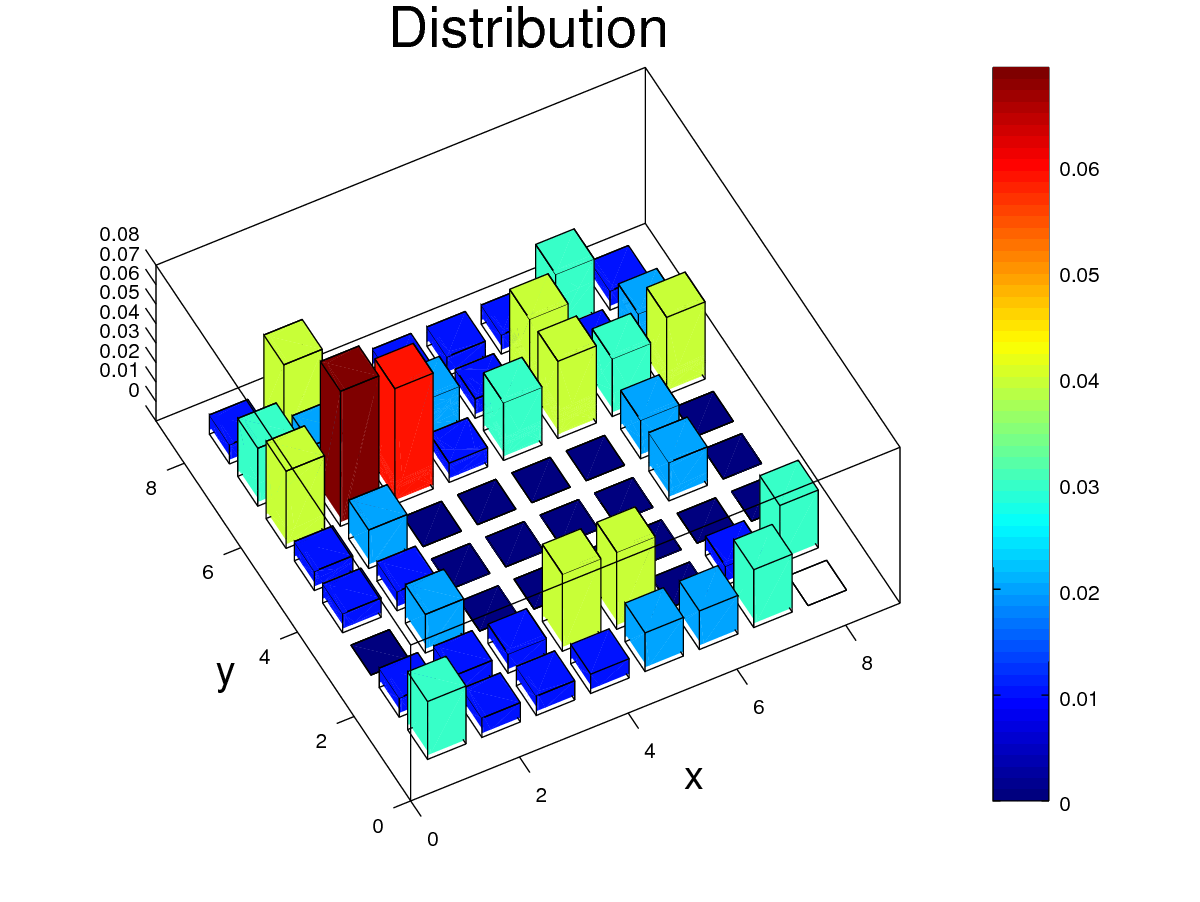
\includegraphics[width=1.0\linewidth]{figures/withHole/figure_Rook_path_n100.png}
     \captionsetup{labelformat=empty}
     \caption*{$n=100$}
   \end{minipage}\hfil
   \begin{minipage}{0.50\textwidth}
     \centering
     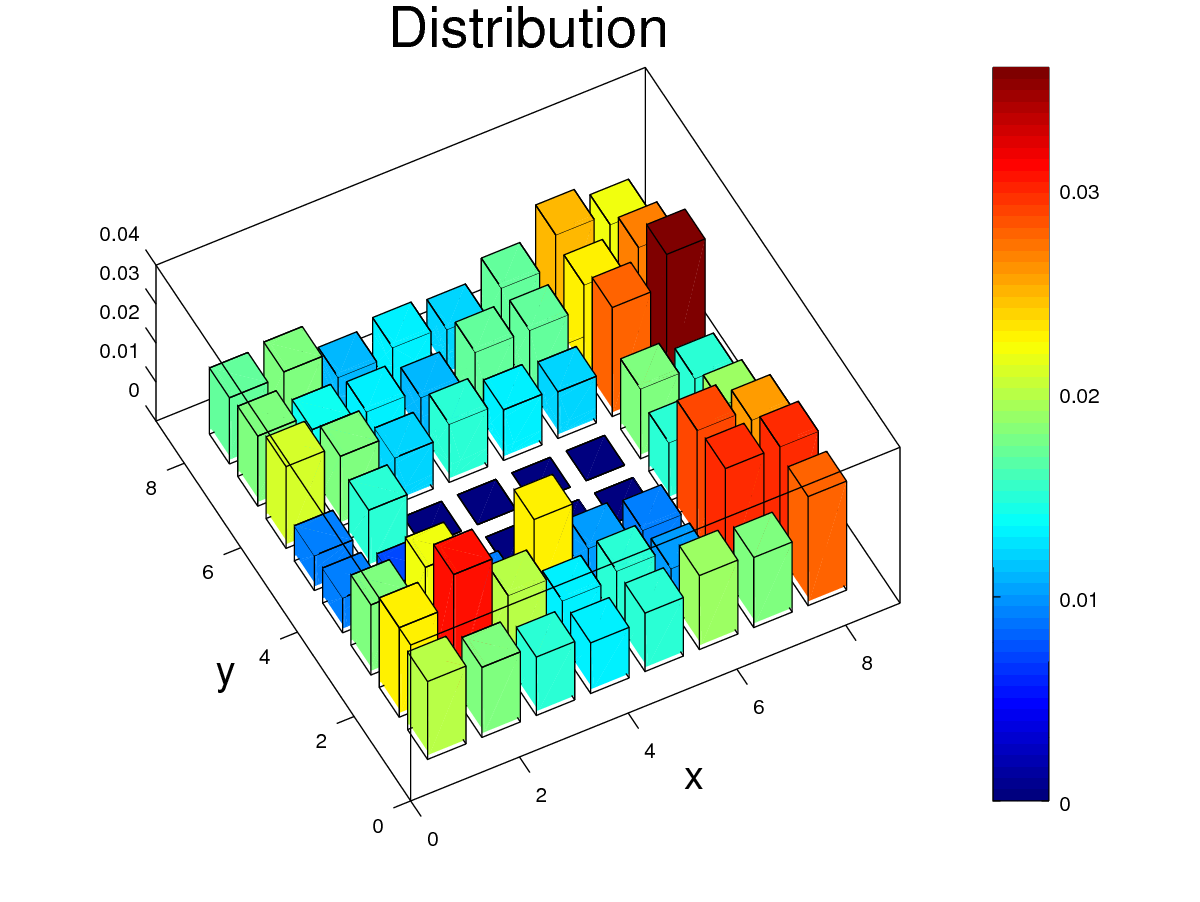
\includegraphics[width=1.0\linewidth]{figures/withHole/figure_Rook_path_n1000.png}
     \captionsetup*{labelformat=empty}
     \caption*{$n=1,000$}
   \end{minipage}\hfil
   \begin{minipage}{0.50\textwidth}
     \centering
     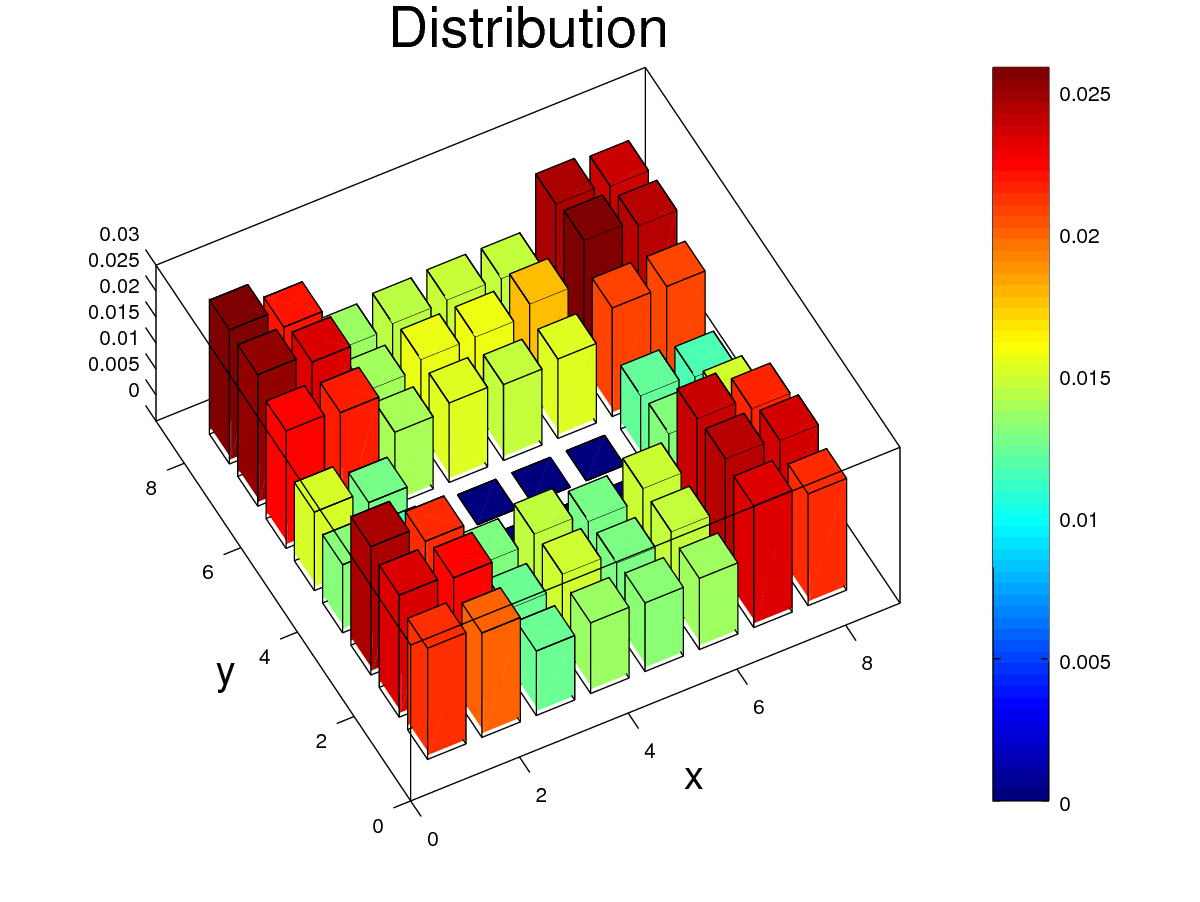
\includegraphics[width=1.0\linewidth]{figures/withHole/figure_Rook_path_n10000.png}
     \captionsetup{labelformat=empty}
     \caption*{$n=10,000$}
    \end{minipage}\hfil
    \begin{minipage}{0.50\textwidth}
     \centering
     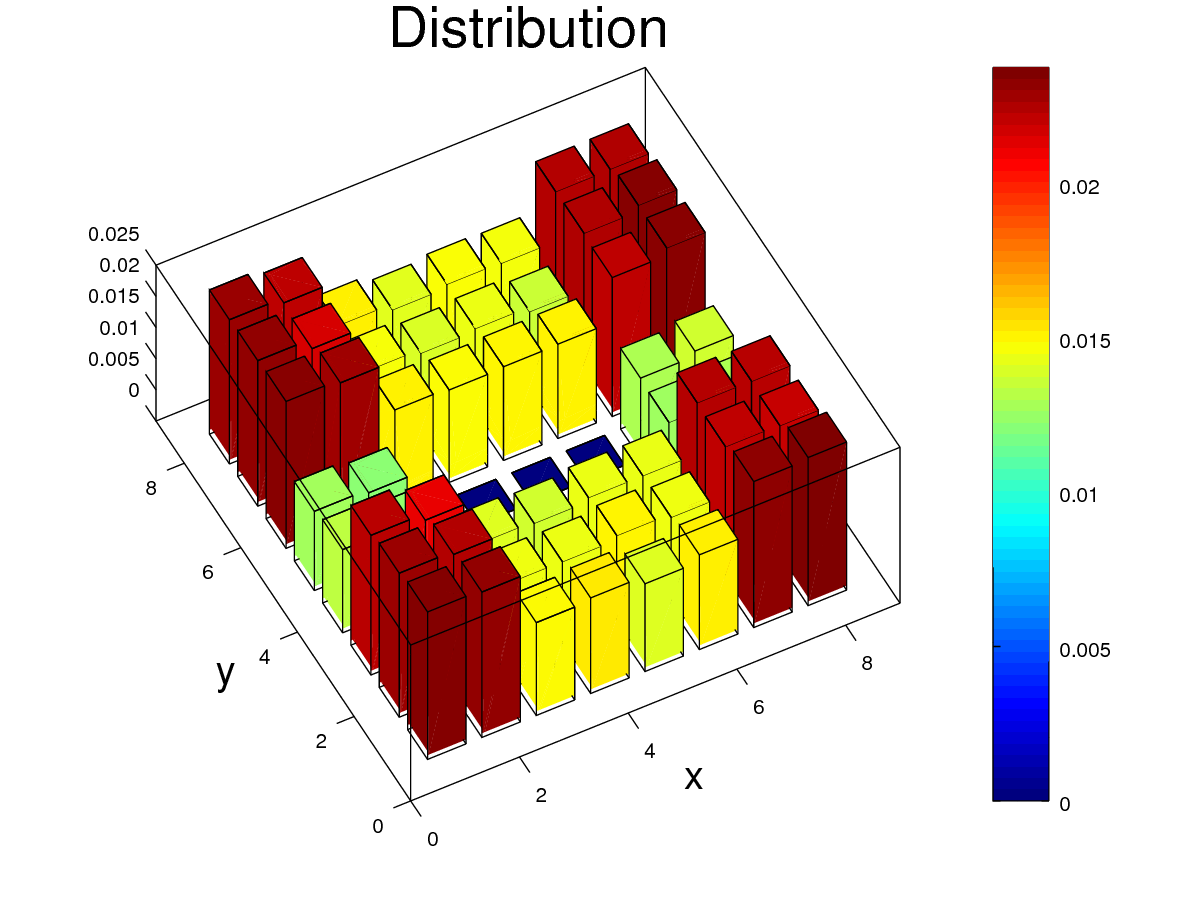
\includegraphics[width=1.0\linewidth]{figures/withHole/figure_Rook_path_n100000.png}
     \captionsetup{labelformat=empty}
     \caption*{$n=100,000$}
   \end{minipage}\hfill
   \begin{minipage}{0.50\textwidth}
     \centering
     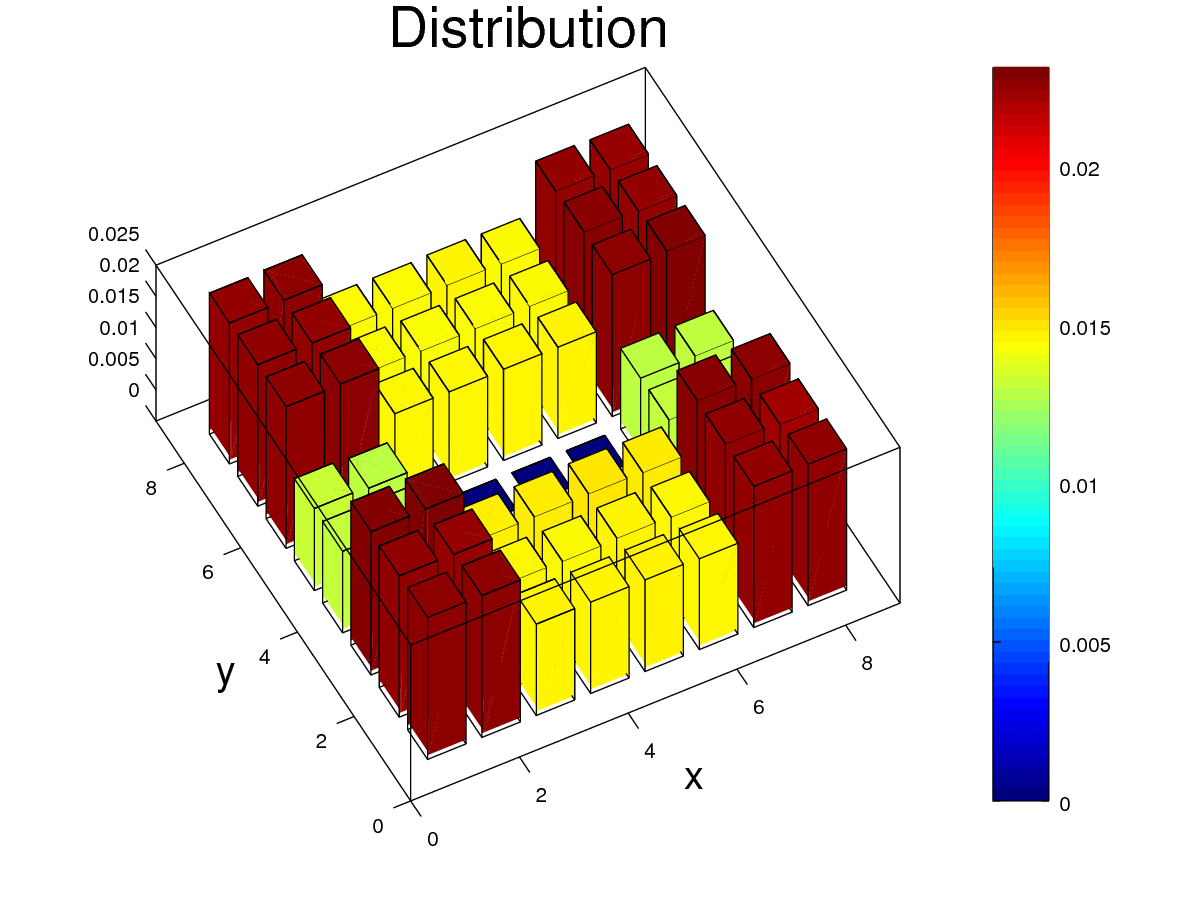
\includegraphics[width=1.0\linewidth]{figures/withHole/figure_Rook_path_n1000000.png}
     \captionsetup{labelformat=empty}
     \caption*{$n=1,000,000$}
   \end{minipage}\hfil
   \begin{minipage}{0.50\textwidth}
     \centering
     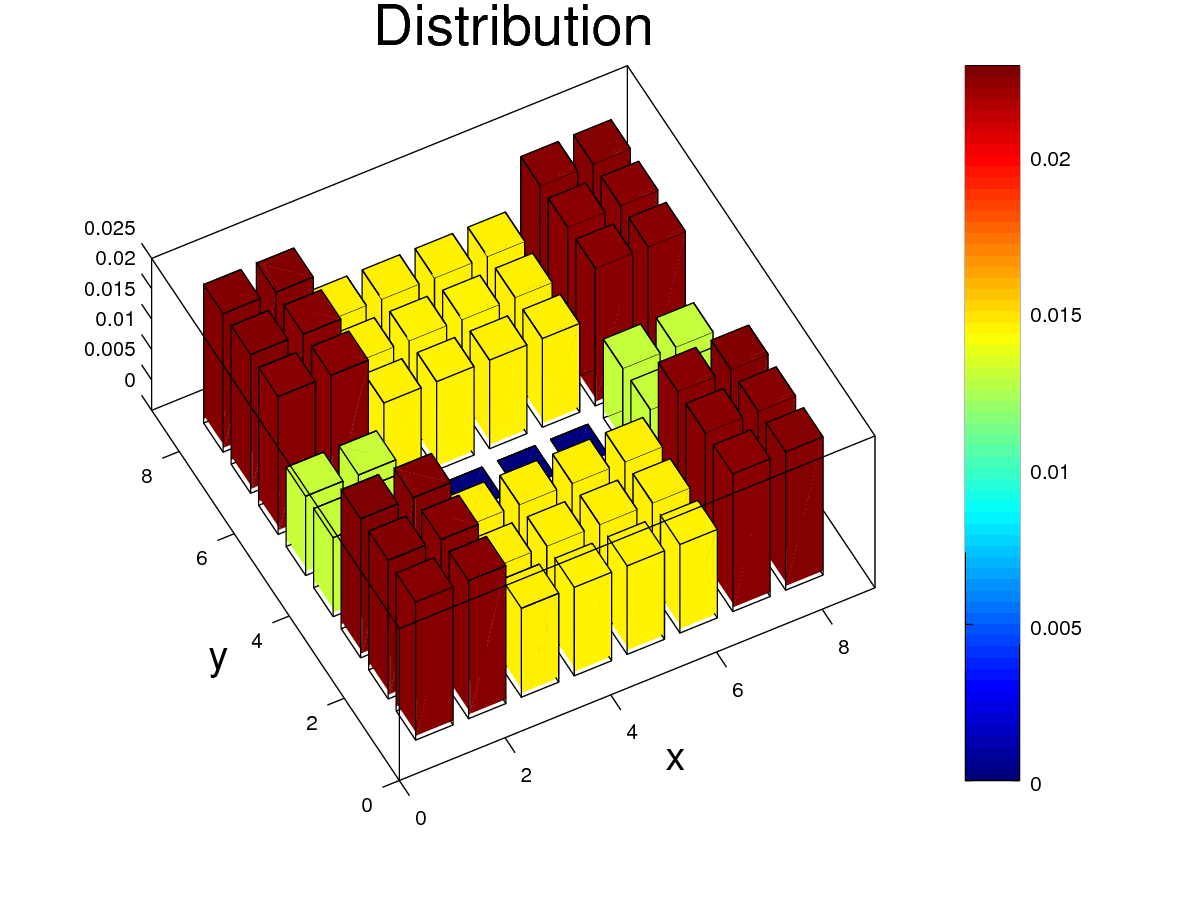
\includegraphics[width=1.0\linewidth]{figures/withHole/figure_Rook_path_n10000000.png}
     \captionsetup{labelformat=empty}
     \caption*{$n=10,000,000$}
    \end{minipage}\hfil
    %\captionsetup{labelformat=empty}
    \caption{Graphs of the probability distribution of the Rook on a board with a hole in the middle; each square on the board is represented by a column (graphs for 5c).}
    \label{plots:graphs_5c1}
\end{figure}





\begin{figure}[!h]
    \centering

\begin{lstlisting}[language=octave]
function probabilities = Rook_path_opt (x0, y0, map, n, directory, save)
  original_map = map;
  
  x = x0;
  y = y0;
  if (map(x,y)!=-1)
    map(x,y) = map(x,y) +1;
  else
    disp('there was a hole...');
    map = RemoveHole(original_map, map);
    probabilities = map./(n+1);
    return;
  endif
  
  xs = zeros(1,n);
  ys = zeros(1,n);
  
  min_n = 100;
  index = 1;
  if (n<min_n)
    xs(index) = x0;
    ys(index) = y0;
    index++;
  endif
  
  for i=1:n
    [x_p1, y_p1] = Rook_move_opt(x,y,map);
    map(x_p1,y_p1) = map(x_p1,y_p1) +1; 
    if (n<min_n) 
      xs(index) = x_p1;
      ys(index) = y_p1;
      index++;
    endif
    x = x_p1;
    y = y_p1;
  endfor
  
  map = RemoveHole(original_map, map);
  
  probabilities = map./(n+1);
  
  if (n<min_n)
    name = strcat(directory,"/figure_Rook_path_n",mat2str(n),"_x",mat2str(x0),"_y",mat2str(y0),".png");
    walkingPlot(xs,ys, map, n, name, save);
  else
    name = strcat(directory,"/figure_Rook_path_n",mat2str(n),".png");
    bar3octave(probabilities, name, save);
  endif
  
  if (save)
    disp(name);
  endif
  
endfunction
\end{lstlisting}

    \caption{The code for the rook path. Comments removed from code to fit to page.}
    \label{code:rook_path}
\end{figure}

\begin{figure}[!h]
    \centering
    \begin{lstlisting}[language=octave]
function avg_steps = Rook_journey_opt (N, map, directory, save)
  
  #the name of the file.
  name = strcat(directory,"/figure_Rook_journey_N",mat2str(N),".png");
  
  #The number of steps for each sample path.
  number_of_steps = zeros(1,N);
  
  #run the simulation for each sample path.
  for path=1:N
    map_copy = map; #get a copy of the board
    x = y = 1; #start from the bottom left
    #increment the number of steps by one
    number_of_steps(path) = number_of_steps(path) +1;
    #increment the count in the map by one
    map_copy(x,y) = map_copy(x,y) +1;
    #For the given point start generating new points
    while(true)
      #this is a new point
      [x_p1, y_p1] = Rook_move_opt(x,y,map_copy);
      #increment the count for that point
      map_copy(x_p1,y_p1) = map_copy(x_p1,y_p1) +1;
      #add a count to the total number of steps
      number_of_steps(path) = number_of_steps(path) +1;
      x = x_p1;
      y = y_p1;
      #if the Rook has gotten to
      #the other end of the board
      #then the path is complete
      if (x==8 && y==8)
        break;
      endif
    endwhile
    
  endfor
  
  #print the name is you are going to save
  if (save)
    disp(name);
  endif
  
  %number_of_steps
  histPlot(number_of_steps, name, save);
  avg_steps = mean(number_of_steps);
  
endfunction
    \end{lstlisting}
    \caption{The code for rook journey.}
    \label{code:rook_journey}
\end{figure}

\begin{figure}[!h]
    \centering
    \begin{lstlisting}[language=octave]
function new_map = RemoveHole (holed_map, prob_map)
  #the map to be returned without any holes.
  new_map = prob_map+(-1)*holed_map;
endfunction
    \end{lstlisting}
    \caption{This function is used to remove holes from the map.}
    \label{code:remove_hole}
\end{figure}


\textbf{Rook Movement Function:}
\begin{lstlisting}[language=octave][!h]
## A valid point from (x0,y0) is generated and returned to
## the caller as x1 and y1.
## x0 - The initial x position the Rook starts at.
## y0 - The initial y position the Rook starts at.
## map - The map of the board, this needs to be an 8X8 matrix
##       and can have -1s where there are holds and 0 everywhere else.
function [x1 y1] = Rook_move_opt (x0, y0, map)

  #initialize the new points.
  x1 = 0;
  y1 = 0;
  
  #if the map at the points given is -1
  #then return x1=-1 and y1=-1.
  if (map(x0,y0)==-1)
    printf('.');
    x1 = -1;
    y1 = -1;
    return;
  endif
  
  #generate a new point using this loop.
  while (true)
    #determines which path to move down
    column_or_row = floor(2*rand())+1;
    rand_xy = floor(8*rand())+1;
    if (column_or_row==1) #take the column
      x1 = x0;
      y1 = rand_xy;
    else #take the row
      x1 = rand_xy;
      y1 = y0;
    endif
    
    #is the square not blocked off and is the piece not in the position
    if (map(x1,y1)!=-1 && (x1!=x0 || y1!=y0))
      
      #was the choice a column
      if (column_or_row==1)
        check_y0 = 0;
        check_y1 = 0;
        if y1>y0 #greater than the previous point
          check_y0 = y0;
          check_y1 = y1;
        else #less than or equal to the previous point
          check_y0 = y1;
          check_y1 = y0;
        endif
        
        #where all of the points up to the proposed point not equal to -1
        if (map(x1, check_y0:check_y1)!=-1)
          break;
        endif
        
      #was the choice a row
      else
        check_x0 = 0;
        check_x1 = 0;
        if x1>x0 #greater than the previous point
          check_x0 = x0;
          check_x1 = x1;
        else #less than or equal to the previous point
          check_x0 = x1;
          check_x1 = x0;
        endif
        
        #where all of the points up to the proposed point not equal to -1
        if (map(check_x0:check_x1, y1)!=-1)
          break;
        endif
        
      endif
      
    else
      #try, try, again
      continue;
    endif
    
  endwhile

endfunction
\end{lstlisting}

\textbf{Function to plot a sample path:}
\begin{lstlisting}[language=octave]
function walkingPlot(xs, ys, map, n, name, save)
  
  subplot(1,2,1);
  plot(xs, ys, "b*-");
  axis ([1, 8, 1, 8], "square");
  title("Rook Path", "fontsize", 27);
  xlabel("x", "fontsize", 19);
  ylabel("y", "fontsize", 19);
  set(gca,'fontsize',20);
  grid on;
  
%  subplot(1,3,2);
%  hist(lengths, "r");
%  title("Histogram of Lengths", "fontsize", 27);
%  xlabel("Steps", "fontsize", 19);
%  ylabel("Count", "fontsize", 19);
%  set(gca,'fontsize',20);
%  grid on;
  
  subplot(1,2,2);
  bar3octave(map./(n+1), name, false);
  
  if (save)
    saveas (1, name);
  endif

endfunction
\end{lstlisting}

\textbf{Function to test the movement algorithm:}
\begin{lstlisting}[language=octave]
## The path of the rook is computed using this function
## x0 - The initial x position the Rook starts at.
## y0 - The initial y position the Rook starts at.
## map - The map of the board, this needs to be an 8X8 matrix
##       and can have -1s where there are holds and 0 everywhere else.
## n - The number of steps to take in the walk.
## directory - The directory to save the figure.
## save - The boolean value to decided if the figure should be saved or not.
function Rook_moveFixedOrigin (x0, y0, map, n, directory, save)
  
  #the name of the graph.
  name = strcat(directory,"/figure_Rook_moveFixedOrigin_N",mat2str(n),"_x", mat2str(x0),"_y", mat2str(y0),".png");
  map_original = map; #a copy of the original map
  #if the piece starts off on a hole do nothing.
  if (map(x0,y0)==-1)
    disp('There was a hole at that point');
  else
    #increment the count at the original point
    map(x0, y0) = map(x0,y0) +1;
    #Generate a bunch of new samples from a fixed origin
    for i=1:n
      [x1, y1] = Rook_move_opt(x0, y0, map); #a new sample square
      map(x1,y1) = map(x1,y1) +1; #increment the count for that square
    endfor
    
    #remove the holes in the map (remove the -1s)
    map = RemoveHole(map_original, map);
    
    #print the name is you are going to save
    if (save)
      disp(name);
    endif
    
    probs_movementFixedOrigin = map./(n+1)
    
    #plot the 3D bar chart
    bar3octave(map./(n+1), name, save);
  endif
  
endfunction

\end{lstlisting}

\textbf{A wrapper class for the main path function:}
\begin{lstlisting}[language=octave]
## this is a simplified version of the Rook_path_opt function.
function probabilities = Rook_path(x0, y0, n)
  map = zeros(8,8); #A board with not holes.
  probabilities = Rook_path_opt(x0, y0, map, n, '', false);
endfunction
\end{lstlisting}

\textbf{A wrapper class for the main movement function:}
\begin{lstlisting}[language=octave]
## A simplified verison of the Rook_move_opt function.
function [x1 y1] = Rook_move(x0, y0)
  map = zeros(8,8); #A board with no holes.
  [x1 y1] = Rook_move_opt(x0, y0, map);
endfunction
\end{lstlisting}


\textbf{The function used to perform the EXTRA CREDIT problem:}
\begin{lstlisting}[language=octave]
function avg_steps = Rook_long_journey (N, map, directory, save)
  
  #the name of the file.
  name = strcat(directory,"/figure_Rook_long_journey_N",mat2str(N),".png");
  
  #The number of steps for each sample path.
  number_of_steps = zeros(1,N);
  
  #run the simulation for each sample path.
  for path=1:N
    has_top_left = false;
    has_top_right = false;
    has_bottom_right = false;
    map_copy = map; #get a copy of the board
    x = y = 1; #start from the bottom left
    #increment the number of steps by one
    number_of_steps(path) = number_of_steps(path) +1;
    #increment the count in the map by one
    map_copy(x,y) = map_copy(x,y) +1;
    #For the given point start generating new points
    while(true)
      #this is a new point
      [x_p1, y_p1] = Rook_move_opt(x,y,map_copy);
      #increment the count for that point
      map_copy(x_p1,y_p1) = map_copy(x_p1,y_p1) +1;
      #add a count to the total number of steps
      number_of_steps(path) = number_of_steps(path) +1;
      x = x_p1;
      y = y_p1;
      
      #booleans for checking if the 
      #Rook has visited all corners
      #other than (1,1)
      if (x==1 && y==8)
        has_top_left = true;
      elseif (x==8 && y==8)
        has_top_right = true;
      elseif (x==8 && y==1)
        has_bottom_right = true;
      endif
      
      #if the Rook has visited all corner and is on
      #(1,1) then break out of the while loop;
      #this path is complete.
      if ((x==1 && y==1) && has_top_left==true && has_top_right==true && has_bottom_right==true) 
        break;
      endif
      
    endwhile
    
  endfor
  
  #print the name is you are going to save
  if (save)
    disp(name);
  endif
  
  %number_of_steps
  histPlot(number_of_steps, name, save);
  avg_steps = mean(number_of_steps);
  
endfunction

\end{lstlisting}


\textbf{A wrapper class for the main journey function:}
\begin{lstlisting}[language=octave]
## A simpler version of the Rook_journey_opt function.
function avg_steps = Rook_journey(N)
  map = zeros(8,8); #A board with no holes
  avg_steps = Rook_journey_opt(N, map, '', false);
endfunction
\end{lstlisting}

\textbf{The main script used to generate all results for the paper:}
\begin{lstlisting}[language=octave]
format short;

disp('+++ test case 1 +++')


%%graph the regular chess board...
directory_regular = 'figures/regular'
save = false
map = zeros(8,8);
GraphAll(map, directory_regular, save, true);


%%graph the chess board with a hole in the middle...
directory_withHole = 'figures/withHole'
save = false
map = zeros(8,8);
map(3:6, 4:5) = -1;
GraphAll(map, directory_withHole, save, true);

%map = zeros(8,8)
%#map(3:6, 4:5) = -1;
%N = 10000
%directory = 'figures'
%save = false
%Rook_moveFixedOrigin(1, 1, map, 10^3, directory, false);
%index = increment(bar, index, count, title);
%average_steps = Rook_journey_opt(N, map, directory, save);
%average_steps = Rook_long_journey(N, map, directory, save)

%map = zeros(8,8);
%map(3:6, 4:5) = -1;
%probabilities = Rook_path_opt(1,1, map, 1000, '', false);
%probabilities
#average_steps = Rook_journey_opt(1000, map, '', false);

%probabilities = Rook_path(1,1, 10^5);
\end{lstlisting}


\textbf{The function used to plot a histogram:}
\begin{lstlisting}[language=octave]
function histPlot (lengths, name, save)

  subplot(1,1,1);
  hist(lengths, 25, "r");
  title("Histogram of Lengths", "fontsize", 27);
  xlabel("Steps", "fontsize", 19);
  ylabel("Count", "fontsize", 19);
  set(gca,'fontsize',20);
  grid on;
  
  if(save)
    saveas(1, name);
  endif
  
endfunction
\end{lstlisting}

\textbf{Our modified 3D bar-chart code to support plotting to a file and plotting to another figure window:}
\begin{lstlisting}[language=octave]
function bar3octave(Z, name, save);

  %
  %**************************************************************
  % Create a 3D bar plot for the input two-dimensional matrix Z.
  % No checking is being done if Z is a 2D matrix.
  %
  % Inputs:
  %    Z: a two-dimensional array (matrix) of real numbers
  %
  % Output:
  %    none
  %
  % Usage:
  %    bar3octave(Z) ... Z a 2D matrix
  %    bar3octave([1 2 3; 4 5 6; 7 8 9])
  %
  % Written by PB, January 21, 2015.
  % (Based on a code by Rody Oldenhuis from
  %  http://stackoverflow.com/questions/24180890/3d-histogram-with-gnuplot-or-octave)
  %**************************************************************
  %

  #graphics_toolkit("fltk")

  %clf;
  hold on;
  view(-27.5, 70);
  %view(3);
  #view ([azimuth elevation])
  
  %# the "nominal" bar (adjusted from cylinder())
  n = 4;
  r = [0.5; 0.5];
  m = length(r);
  theta = (0:n)/n*2*pi + pi/4;

  x0 = r * cos(theta);
  y0 = r * sin(theta);
  z0 = (0:m-1)'/(m-1) * ones(1,n+1);

  %# get data for current colormap
  map = colormap; #("jet")
  Mz = max(Z(:));
  mz = min(Z(:));
  
  % Each "bar" is 1 surf and 1 patch
  for ii = 1:size(Z,1)
      for jj = 1:size(Z,2)

          % Get color (linear interpolation through current colormap)
          cI = (Z(ii,jj)-mz)*(size(map,1)-1)/(Mz-mz) + 1;
          fC = floor(cI);
          cC = ceil(cI);
          color = map(fC,:) + (map(cC,:) - map(fC,:)) * (cI-fC);
          
          % Translate and rescale the nominal bar
          x = x0+ii;
          y = y0+jj;
          z = z0*Z(ii,jj);

          % Draw the bar
          surf(x,y,z, 'Facecolor', color)
          patch(x(end,:), y(end,:), z(end,:), color)

      end
  end

  colorbar;
  caxis([mz Mz]);
  axis([0, size(Z,1)+1, 0, size(Z,2)+1]);
  
  title("Distribution", "fontsize", 27);
  xlabel("x", "fontsize", 19);
  ylabel("y", "fontsize", 19);

  if (save)
    saveas (1, name);
  endif
  
  hold off;
  
endfunction

\end{lstlisting}


\textbf{The function used to generate all graphs for a given map:}
\begin{lstlisting}[language=octave]
## Graphs all plots needed for the paper.
## map - The map of the board, this needs to be an 8X8 matrix
##       and can have -1s where there are holds and 0 everywhere else.
## directory - The directory to save the figure.
## save - The boolean value to decided if the figure should be saved or not. 
## runtime: true for long and false for short. If true a few more 
##          long running computations will be run.
function GraphAll (map, directory, save, runtime)
  
  title = 'generating all Graphs';
  bar = waitbar(0.0, title);
  count = 23;
  if (runtime)
    count = count -2;
  endif
  index = 1;
  
  %firet set of graphs. These test the distribution of values
  % starting from various fixed positions.
  # Test cases to show that the movement function is
  # producing equally weighted samples for the next move.
  Rook_moveFixedOrigin(1, 1, map, 10^6, directory, save);
  index = increment(bar, index, count, title);
  
  Rook_moveFixedOrigin(8, 8, map, 10^6, directory, save);
  index = increment(bar, index, count, title);
  
  Rook_moveFixedOrigin(4, 4, map, 10^6, directory, save);
  index = increment(bar, index, count, title);
  
  Rook_moveFixedOrigin(1, 4, map, 10^6, directory, save);
  index = increment(bar, index, count, title);
  
  Rook_moveFixedOrigin(4, 1, map, 10^6, directory, save);
  index = increment(bar, index, count, title);
  
  %second set of graphs. These functions generate the graphs
  %for the paths.
  #Example paths starting from various places on the board.
  probabilities = Rook_path_opt(1,1, map, 5, directory, save);
  index = increment(bar, index, count, title);
  
  probabilities = Rook_path_opt(1,1, map, 10, directory, save);
  index = increment(bar, index, count, title);
  
  probabilities = Rook_path_opt(1,1, map, 25, directory, save);
  index = increment(bar, index, count, title);
  
  
  probabilities = Rook_path_opt(8,8, map, 5, directory, save);
  index = increment(bar, index, count, title);
  
  probabilities = Rook_path_opt(8,8, map, 10, directory, save);
  index = increment(bar, index, count, title);
  
  probabilities = Rook_path_opt(8,8, map, 25, directory, save);
  index = increment(bar, index, count, title);
  
  
  probabilities = Rook_path_opt(4,1, map, 5, directory, save);
  index = increment(bar, index, count, title);
  
  probabilities = Rook_path_opt(4,1, map, 10, directory, save);
  index = increment(bar, index, count, title);
  
  probabilities = Rook_path_opt(4,1, map, 25, directory, save);
  index = increment(bar, index, count, title);
  
  %third set of graphs. These methods generate 3d bar charts
  %for various n values starting from the first square on the
  %board.
  # (5a) The probabilities for each of the squares on the board.
  x0 = 1;
  y0 = 1;
  probabilities = Rook_path_opt(x0,y0, map, 10^2, directory, save);
  index = increment(bar, index, count, title);
  
  probabilities = Rook_path_opt(x0,y0, map, 10^3, directory, save);
  index = increment(bar, index, count, title);
  
  probabilities = Rook_path_opt(x0,y0, map, 10^4, directory, save);
  index = increment(bar, index, count, title);
  
  probabilities = Rook_path_opt(x0,y0, map, 10^5, directory, save);
  index = increment(bar, index, count, title);
  
  if (runtime)
    probabilities = Rook_path_opt(x0,y0, map, 10^6, directory, save);
    index = increment(bar, index, count, title);
    
    probabilities = Rook_path_opt(x0,y0, map, 10^7, directory, save);
    index = increment(bar, index, count, title)
    probabilities
  endif
  
  %the fourth set of graphs. This function generates 1000 paths and
  %averages them to find to find the average number of steps it takes
  %to get from the lower left to the upper right corner.
  # (5b) The average number of steps needed to get from one
  # corner to the next.
  average_steps = Rook_journey_opt(10000, map, directory, save);
  index = increment(bar, index, count, title);
  
  close(bar);
  close
  
  disp('average_steps: ');
  disp(average_steps);

endfunction

function iii = increment(bar, index, count, title)
  waitbar(index/count, bar, title);
  iii = index + 1;
  clf;
endfunction
\end{lstlisting}

\textbf{}
\begin{lstlisting}[language=octave]

\end{lstlisting}

\textbf{}
\begin{lstlisting}[language=octave]

\end{lstlisting}


\textbf{}
\begin{lstlisting}[language=octave]

\end{lstlisting}

\textbf{}
\begin{lstlisting}[language=octave]

\end{lstlisting}




\newpage
\section{Bibliography}
	Project 2 packet written by Pavel Belik \par
	gnu.org \par
	


\end{document}

%------------------------------------------------------------------------------
% End of journal.tex
%------------------------------------------------------------------------------
